\chapter{Simulation design \& Results} \label{chapter:simul}
%3. MAIN SECTION(s)
%Include description of the overall design, flowcharts for sections of the design, finite state machines for separate sections as needed.

\section{Introduction} \label{sec:simul:intro}
This chapter is concerned with the overall design and execution of the experiments conducted in this project. It begins with basic investigations to gain an understanding of YouTube video streaming. Section \ref{sec:simul:ping} shows results when pinging YouTube. These results are informative in running a data collection experiment with \textit{Wireshark} in Section \ref{sec:simul:wireshark}. In light of the information collected in the foregoing sections, Section \ref{sec:simul:riverbed} describes the Riverbed Modeler scenarios implemented in this project and presents the simulation results. Finally, Section \ref{sec:summary} concludes this chapter.

\section{Pinging YouTube} \label{sec:simul:ping}
The URL \url{youtube.com} was pinged to have a realistic idea of the Round Trip Times (\gls{RTT}s). The \gls{IPv6} address for the YouTube server is \verb|2607:f8b0:400a:801::200e| as can be seen in the screenshot in Figure \ref{fig:sim:ping}.

\begin{figure}[H]
	\centering
	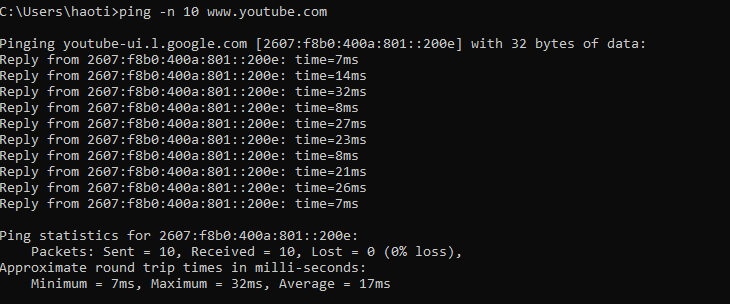
\includegraphics[scale=0.8]{Figures/image1.png}
	\caption{Windows command window: pinging YouTube}
	\label{fig:sim:ping}
\end{figure}

The \gls{RTT} values ranged from $7~\mathrm{ms}$ to $32~\mathrm{ms}$ with an average of $17~\mathrm{ms}$. A \textit{whois} domain lookup done on \url{www.arin.net/whois} shows that the owner of this server is \textit{Google LLC}. This is expected since Google is the owner of YouTube.

\section{Wireshark data collection} \label{sec:simul:wireshark}
\textit{Wireshark} was used to sniff the packets while streaming a 1080p YouTube video using a \gls{WiFi} connection. This was instructive in understanding how YouTube implements video streaming. Since YouTube is known to be an \gls{HTTP} application, port 80 was used to filter the data traffic during packet sniffing.

Figure \ref{fig:sim:w1} shows the Wireshark trace recorded when a YouTube video was streamed.

\begin{figure}[H]
	\centering
	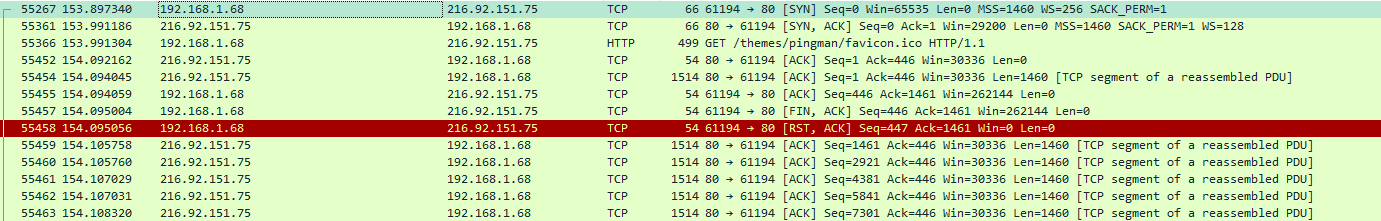
\includegraphics[scale=0.45]{Figures/image3.png}
	\caption{Wireshark trace of TCP connection with server}
	\label{fig:sim:w1}
\end{figure}

Once the user starts playing the video, the socket from their computer tries to make a \gls{TCP} connection with the socket port number 80 (which belongs to YouTube's server side socket). After the connection is established, the client's computer sends an \gls{HTTP} Get message to the YouTube server. This is followed by the server transferring streaming packets to the client's computer.

\begin{figure}[H]
	\centering
	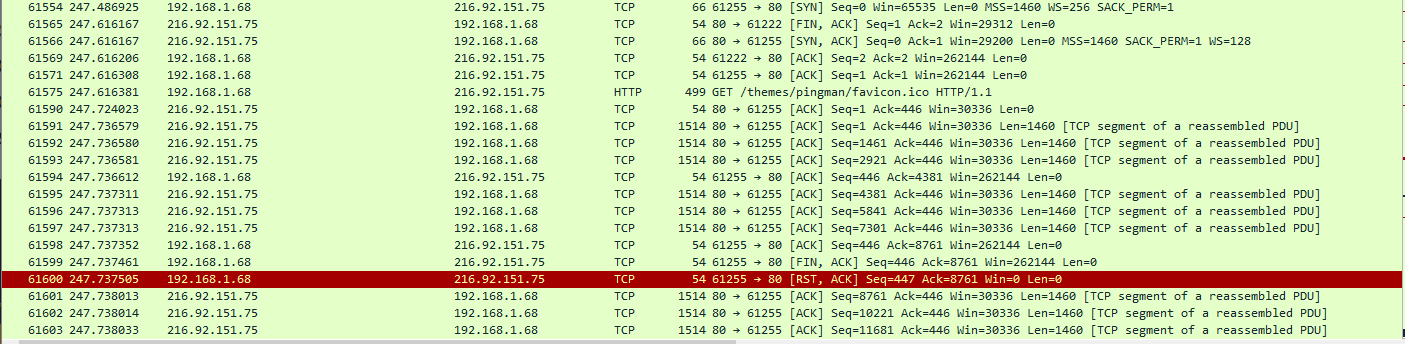
\includegraphics[scale=0.45]{Figures/image2.png}
	\caption[Wireshark trace of TCP connection with YouTube server]{Wireshark trace of \gls{TCP} connection with server}
	\label{fig:sim:w2}
\end{figure}

As can be seen from Figure \ref{fig:sim:w2}, YouTube, as an \gls{HTTP} application, provides reliable video streaming through using \gls{TCP} as transport protocol because of its reliable data transfer  characteristic. The \gls{TCP} protocol allows the receiver to buffer the data packets sent from the streaming server.

\section{Riverbed Modeler simulations} \label{sec:simul:riverbed}
%\hl {Please add an introductory paragraph which states the configuration of the scenario used. Base it on previous reports. Need to provide parameters and values chosen for them. Screenshot of the physical layout on riverbed modeler. duration of the simulation is 1 hour. why did you use 1 hour. explain the choice of data rate.}
%
%explain the rationale behind having 4 scenarios.
%
%the reason why we do not put more work stations in the local area network is because too many workstations will cause the simulation time becomes very short. We would rather to have a more realistic simulation time, for example, one hour, instead of putting lots of workstations in then local area network

YouTube streaming sessions usually last for one hour. Therefore we set the duration of our Riverbed Modeler simulations to one hour. However, as a consequence of the long simulation duration, we were not allowed on include additional work stations in the \gls{WLAN}s we simulated. We opted for a longer simulation duration over supporting additional users to ensure that our results are more comparable to a real-life user streaming YouTube videos on \gls{WiFi} in a residence.

This section presents simulations done in Riverbed Modeler. Four scenarios are developed in this work:
\begin{itemize}
	\item Scenario 1 in Subsection \ref{subsec:riverbed:1} investigates how three different types of browsing profiles (namely light browsing, heavy browsing and video streaming) affect the \gls{QoS} enjoyed by the \gls{WiFi} client.
	\item Scenario 2 uses two video streaming resolutions to find how they affect the throughput and average delay experienced by a \gls{WiFi} client.	
	\item Scenario 4 in Subsection \ref{subsec:riverbed:3} investigates three aspects: \begin{itemize}
		\item the impact of the \gls{WiFi} technology (either of \gls{IEEE802}g and n) employed.
		\item the effect of the chosen frequency band employed.
		\item the effect of varying the data rate.
	\end{itemize}
\item Scenario 4 in Subsection \ref{subsec:riverbed:4} considers the effect of varying the range from the \gls{WiFi} client to the access point.
\end{itemize}

These four scenarios were selected to explore the breadth of the experience of a single client browsing on the Internet and streaming YouTube videos in their residence using a \gls{WiFi} network.

\subsection{Scenario 1: Light browsing, heavy browsing \& video streaming} \label{subsec:riverbed:1}
\subsubsection{Topology} \label{subsubsec:1:topo}
The topology in scenario 1 makes use of wireless LAN (\gls{WLAN}) workstation fixed nodes. The router used is a \gls{WLAN} Ethernet router which is connected to the server by an 10000BaseX Ethernet link. The distance between the router and application nodes are around ten to fifteen meters. The three application nodes are equidistant from the router. The effect of the range between the router and server is not considered during this simulation. Figure \ref{fig:1:topo} shows the topology implemented in scenario 1.

\begin{figure}[H]
	\centering
	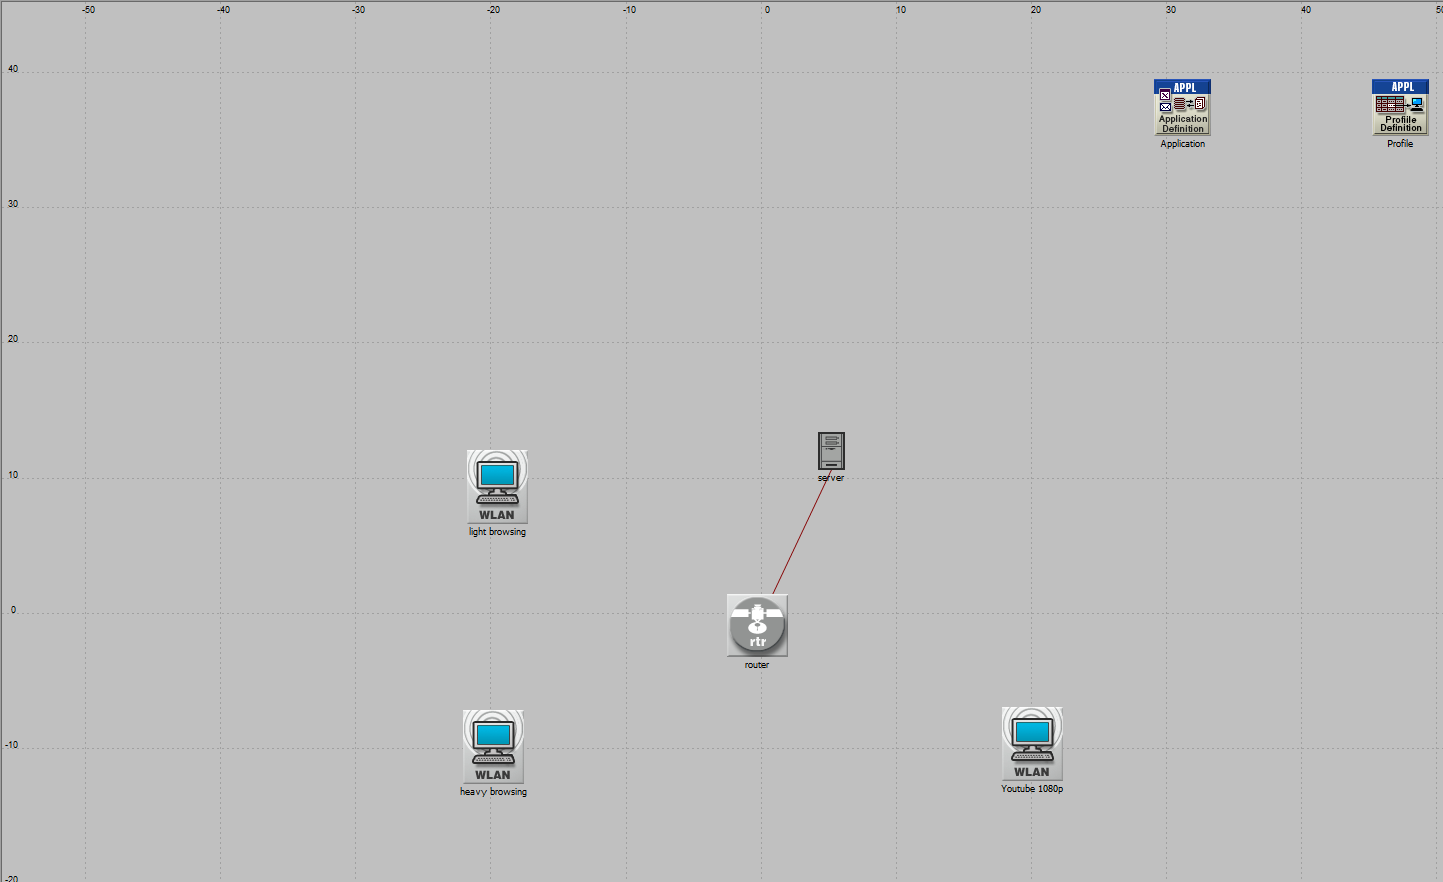
\includegraphics[scale=0.3]{Figures/amantianrenamed/Scenarioonetopology.png}
	\caption{Scenario 1: topology}
	\label{fig:1:topo}
\end{figure}

The BSS Identifier is set to one for both router and wireless LAN workstations so that these wireless LAN workstations can recognize that the router and workstations are in the same local area network. The physical characteristics and data rate are set to \gls{IEEE802}n $2.4~\mathrm{GHz}$ and $65~\mathrm{Mbps}$ (base)/$600~\mathrm{Mbps}$ for both router and wireless workstations in this scenario. We will implement the effect of physical characteristics and data rate in the later scenario.

\begin{figure}[H]
	\centering
	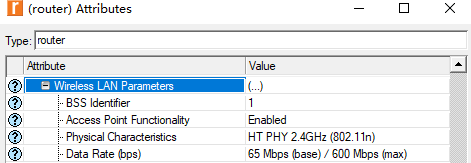
\includegraphics[scale=0.54]{Figures/amantianrenamed/ScenariooneWirelessLanParametersofrouter.png}
	\caption[Wireless LAN parameters of router]{\gls{WLAN} parameters of router}
	\label{fig:1:wlan:para}
\end{figure}

Figure \ref{fig:1:wlan:para} shows the wireless LAN parameters that we set for the router. 

Setting the number of spatial streams to more than 1 and shorter guard intervals will result in higher physical data rate. To get a high physical data rate in this scenario, we set the number of spatial streams to 2 and the Guard Interval (GI) to a short time period of $400~\mathrm{ns}$ under \gls{WLAN} high throughput parameters, as can be seen in Figure \ref{fig:1:wlan:hi}. These two configurations lead to a physical data rate of $57.8~\mathrm{Mbps}$ according to Table 20-30 in \gls{IEEE802}n-2009 \cite{ieee80211n}. We also enabled the Greenfield Operation attribute. This implies that \gls{WLAN} nodes are allowed to a shorter physical layer header format and therefore resulting in higher throughput.

\begin{figure}[H]
	\centering
	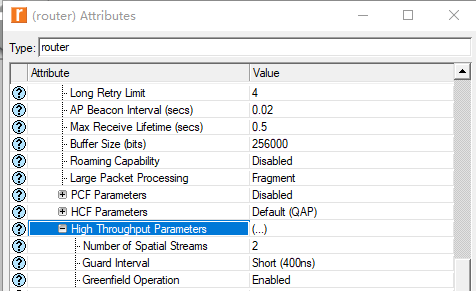
\includegraphics[scale=0.59]{Figures/amantianrenamed/ScenariooneHighThroughputParametersoflocalareanetwork.png}
	\caption{High throughput parameters of Local Area Network}
	\label{fig:1:wlan:hi}
\end{figure}


\subsubsection{Light browsing} \label{subsubsec:light}
The \gls{WLAN} user is first simulated for light browsing, which consumes less system resources. We can see how the profile was configured in Figure \ref{fig:simul:riverbed:light:1}, where we chose the object size as 10,000 bytes with uniform interval between 100 bytes and 4000 bytes. Also we set only one object to be contained in a page  with normal distribution having mean of 10 objects and variance 5 objects. 

\begin{figure}[H]
	\centering
	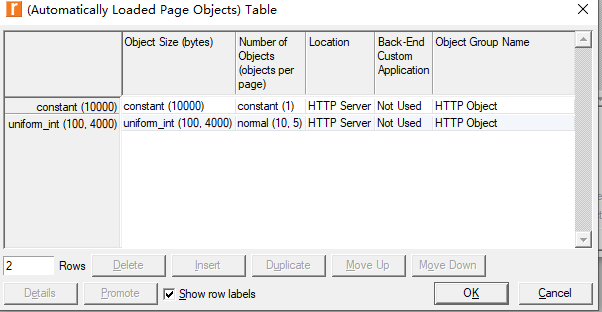
\includegraphics[scale=0.54]{Figures/amantianrenamed/ScenariooneLightbrowsingobjectsize.png}
	\caption{Light browsing scenario: setting object size}
	\label{fig:simul:riverbed:light:1}
\end{figure}

Figure \ref{fig:simul:riverbed:light:2} shows the \gls{HTTP} table for light browsing, which shows that the page inter-arrival time is exponentially distributed with a rate parameter of $720~\mathrm{s}$ by default.
\begin{figure}[H]
	\centering
	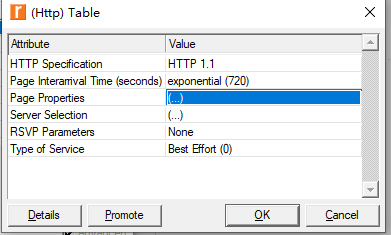
\includegraphics[scale=0.62]{Figures/amantianrenamed/ScenariooneHttpapplicationtableforlightbrowsing.png}
	\caption[Light browsing scenario: HTTP application table]{Light browsing scenario: \gls{HTTP} application table}
	\label{fig:simul:riverbed:light:2}
\end{figure}

Figure \ref{fig:simul:riverbed:light:3} shows the profile setup employed for light browsing.

\begin{figure}[H]
	\centering
	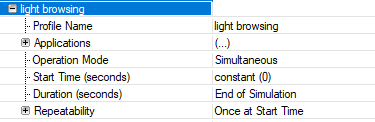
\includegraphics[scale=0.6]{Figures/amantianrenamed/ScenariooneLightBrowsingProfilesetup.png}
	\caption{Light browsing scenario: profile setup}
	\label{fig:simul:riverbed:light:3}
\end{figure}

Figure \ref{fig:simul:riverbed:light:4} shows a plot of the \gls{WLAN} throughput for this scenario.

\begin{figure}[H]
	\centering
	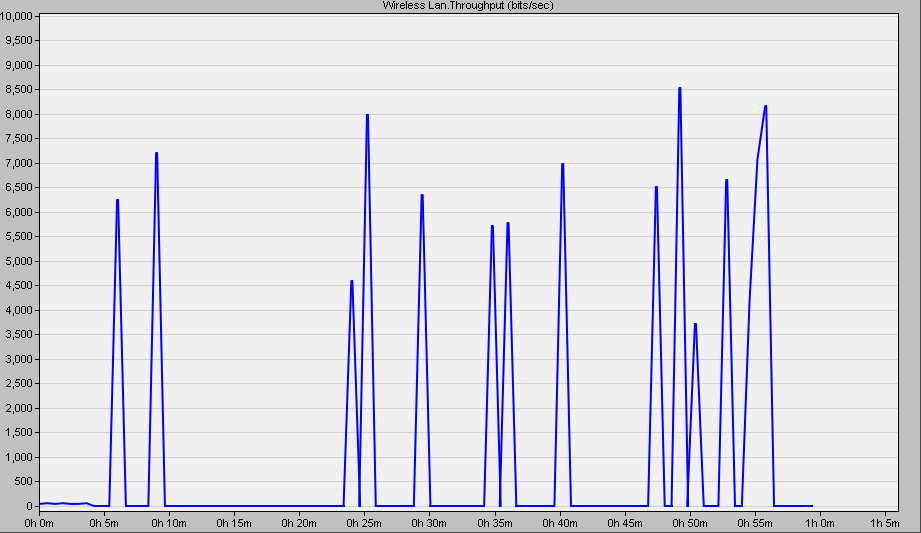
\includegraphics[scale=0.42]{Figures/amantianrenamed/ScenariooneThroughputofLightbrowsing.png}
	\caption{Light browsing scenario: throughput plot}
	\label{fig:simul:riverbed:light:4}
\end{figure}

\subsubsection{Heavy browsing} \label{subsubsec:heavy}
In the heavy browsing scenario, the object size was chosen to be larger (20,000 bytes versus 10,000 bytes in the light browsing scenario in Subsection \ref{subsubsec:light}) and the page inter-arrival time was decreased (more pages are browsed per unit time). As can be seen in Figure \ref{fig:simul:riverbed:heavy:1}, the intervals are uniformly distributed between 5,000 bytes and 15,000 bytes. In a similar vein to the light browsing scenario, we set only one object to be contained in a page, according to a normal distribution with mean 10 objects and variance 5 objects.

\begin{figure}[H]
	\centering
	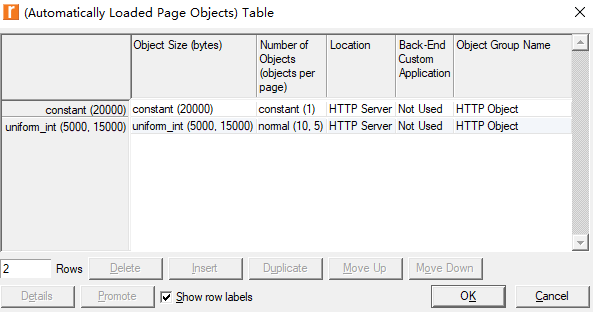
\includegraphics[scale=0.6]{Figures/amantianrenamed/ScenariooneHeavybrowsingobjectsize.png}
	\caption{Heavy browsing scenario: setting object size}
	\label{fig:simul:riverbed:heavy:1}
\end{figure}

Figure \ref{fig:simul:riverbed:heavy:2} shows the application table for heavy browsing, which shows that the page inter-arrival time is exponentially distributed with a rate parameter of 60 seconds.

\begin{figure}[H]
	\centering
	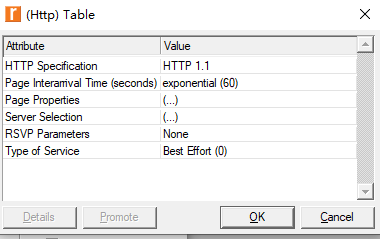
\includegraphics[scale=0.6]{Figures/amantianrenamed/ScenariooneHttpapplicationtableforheavybrowsing.png}
	\caption[Heavy browsing scenario: HTTP application table]{Heavy browsing scenario: \gls{HTTP} application table}
	\label{fig:simul:riverbed:heavy:2}
\end{figure}

Figure \ref{fig:simul:riverbed:heavy:3} shows the profile setup employed for heavy browsing.

\begin{figure}[H]
	\centering
	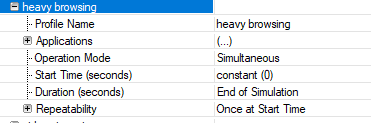
\includegraphics[scale=0.6]{Figures/amantianrenamed/ScenariooneHeavyBrowsingProfilesetup.png}
	\caption{Heavy browsing scenario: profile setup}
	\label{fig:simul:riverbed:heavy:3}
\end{figure}

Figure \ref{fig:simul:riverbed:heavy:4} shows a plot of the \gls{WLAN} throughput for this scenario.

\begin{figure}[H]
	\centering
	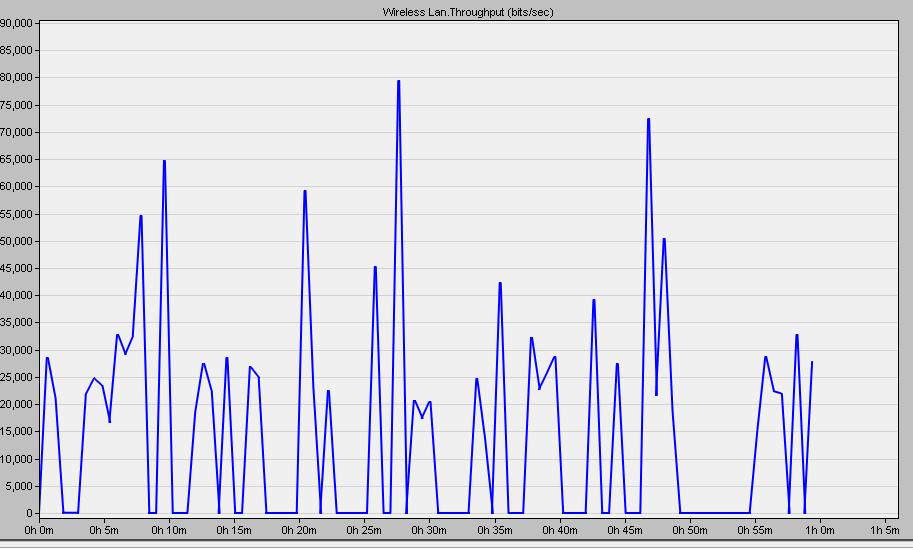
\includegraphics[scale=0.42]{Figures/amantianrenamed/ScenariooneThroughputofHeavybrowsing.png}
	\caption{Light browsing scenario: throughput plot}
	\label{fig:simul:riverbed:heavy:4}
\end{figure}

\subsubsection{Video streaming} \label{subsubsec:video}
In the video streaming scenario, the \gls{HTTP} definition was changed to video browsing and the page inter-arrival time rate parameter was set to $360~\mathrm{s}$. The latter was chosen such that it is shorter than that ($720~\mathrm{s}$) of the light browsing scenario in Subsection \ref{subsubsec:light} and longer than that ($60~\mathrm{s}$) of the heavy browsing scenario in Subsection \ref{subsubsec:heavy}.

For the short video, we set object size to 1000 bytes as can be seen in Figure \ref{fig:simul:riverbed:video:1}. We can expect that the throughput of video streaming to be higher than light and heavy browsing. This is because video streaming requires higher data usage due to larger file sizes.

\begin{figure}[H]
	\centering
	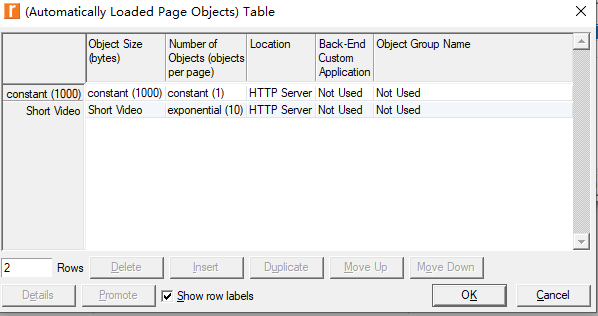
\includegraphics[scale=0.54]{Figures/amantianrenamed/ScenariooneVideoStreamingobjectsize.png}
	\caption{Video streaming scenario: setting object size}
	\label{fig:simul:riverbed:video:1}
\end{figure}

Figure \ref{fig:simul:riverbed:video:2} shows the application table for video streaming, which shows that the page inter-arrival time is exponentially distributed with a rate parameter of 360 seconds.

\begin{figure}[H]
	\centering
	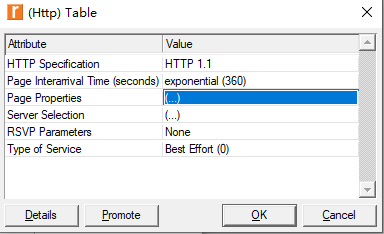
\includegraphics[scale=0.6]{Figures/amantianrenamed/ScenarionHttpapplicationtablevideostreaming.png}
	\caption[Video streaming scenario: HTTP application table]{Video streaming scenario: \gls{HTTP} application table}
	\label{fig:simul:riverbed:video:2}
\end{figure}

Figure \ref{fig:simul:riverbed:video:3} shows the profile setup employed for heavy browsing.

\begin{figure}[H]
	\centering
	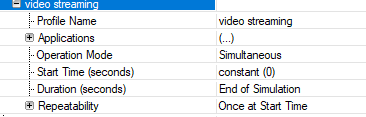
\includegraphics[scale=0.6]{Figures/amantianrenamed/ScenariooneVideostreamingProfileetup.png}
	\caption{Video streaming scenario: profile setup}
	\label{fig:simul:riverbed:video:3}
\end{figure}

Figure \ref{fig:simul:riverbed:video:4} shows a plot of the \gls{WLAN} throughput for this scenario.

\begin{figure}[H]
	\centering
	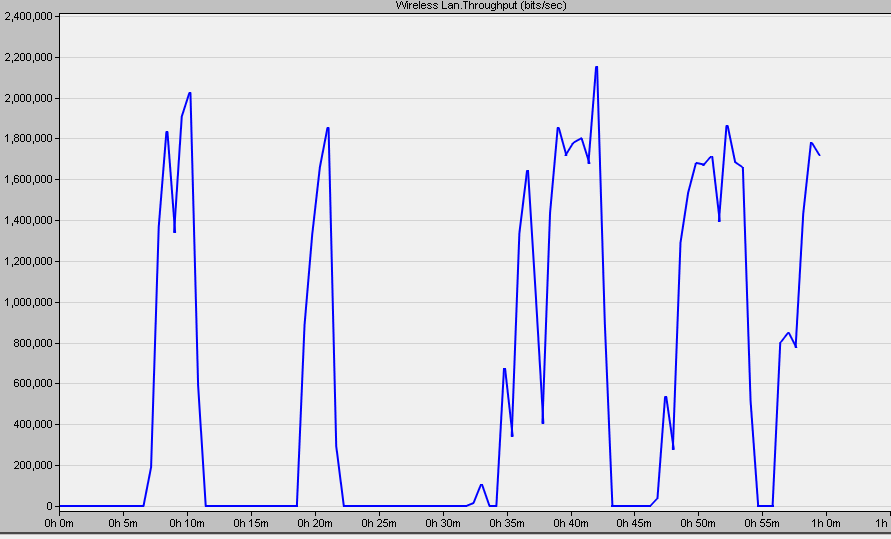
\includegraphics[scale=0.47]{Figures/amantianrenamed/ScenarioThroughputvideostreaming.png}
	\caption{Video streaming scenario: throughput plot}
	\label{fig:simul:riverbed:video:4}
\end{figure}

\subsubsection{Summary of Scenario 1} \label{subsubsec:1:summary}
Based on the work done in Subsections \ref{subsubsec:light}, \ref{subsubsec:heavy} and \ref{subsubsec:video}, we now summarize the results of scenario 1. As can be seen in Figure \ref{subsubsec:1:summary:through}, the average throughput of heavy browsing is more than 8 times higher than that of light browsing. This result may seem intuitive and even though it is logical, its purpose is to serve as a sanity check in our work in this project. 

\begin{figure}[H]
	\centering
	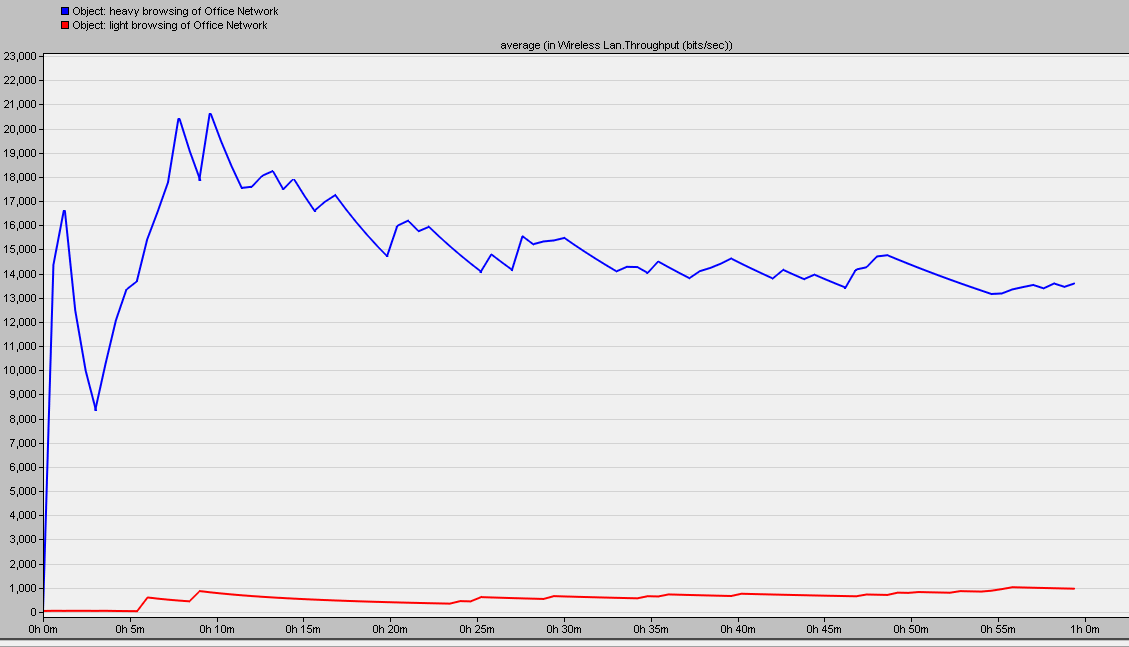
\includegraphics[scale=0.35]{Figures/amantianrenamed/ScenarioAveragelightheavybrowsing.png}
	\caption[Scenario 1: comparison of average throughput]{Comparison of average throughput of light browsing and heavy browsing. The blue graph represents heavy browsing while the red graph represents light browsing.}
	\label{subsubsec:1:summary:through}
\end{figure}

The reason for this significant difference is that heavy browsing has larger object size and shorter page inter-arrival time as compared to light browsing.

Furthermore, Figure \ref{subsubsec:1:summary:throughput} compares the average throughput of video streaming to that of the other two cases. This figure was included separately from Figure \ref{subsubsec:1:summary:through} because it does not show clearly the difference between the throughput of light browsing and heavy browsing.

\begin{figure}[H]
	\centering
	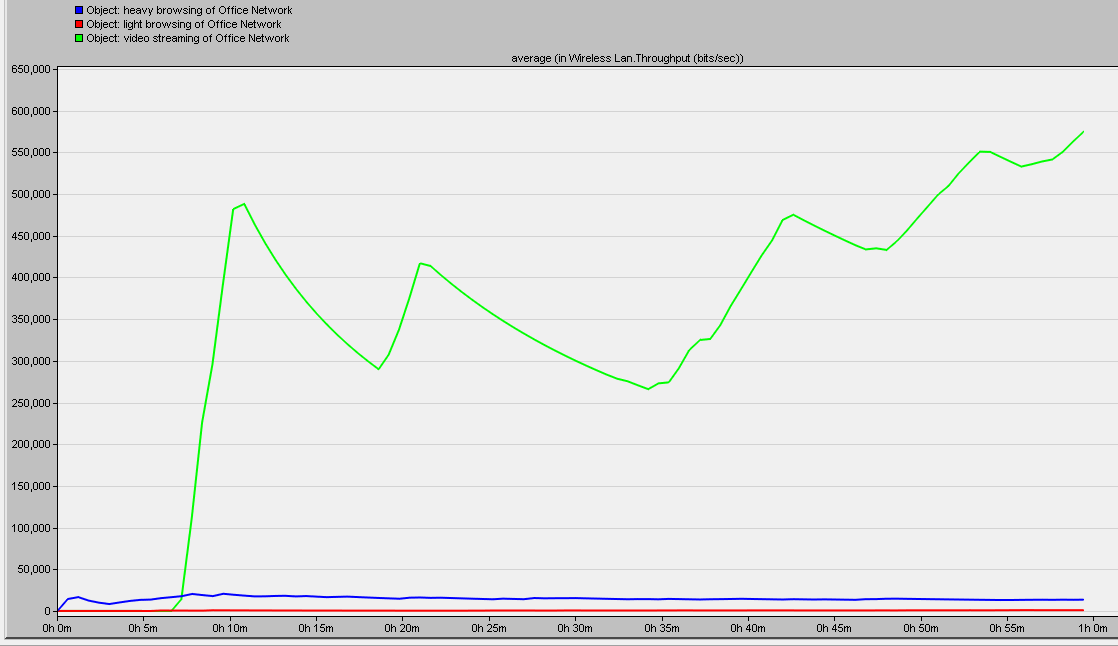
\includegraphics[scale=0.35]{Figures/amantianrenamed/ScenariooneAverageoverlaidthroughputbetweenvideostreaminglightbrowsingandheavybrowsing.png}
	\caption[Scenario 1: comparison of average throughput]{Comparison of average throughput of light browsing, heavy browsing and video streaming. The green trendline represents video streaming.}
	\label{subsubsec:1:summary:throughput}
\end{figure}

Figure \ref{subsubsec:1:summary:throughput} shows that the average throughput of video streaming is more than 10 times higher than that of the two other cases. This intuitive result is explained by the fact that video streaming entails transferring a much larger volume of data than regular web browsing.

Figure \ref{subsubsec:1:summary:delay1} compares the average delay in the three cases considered for Scenario 1.

\begin{figure}[H]
	\centering
	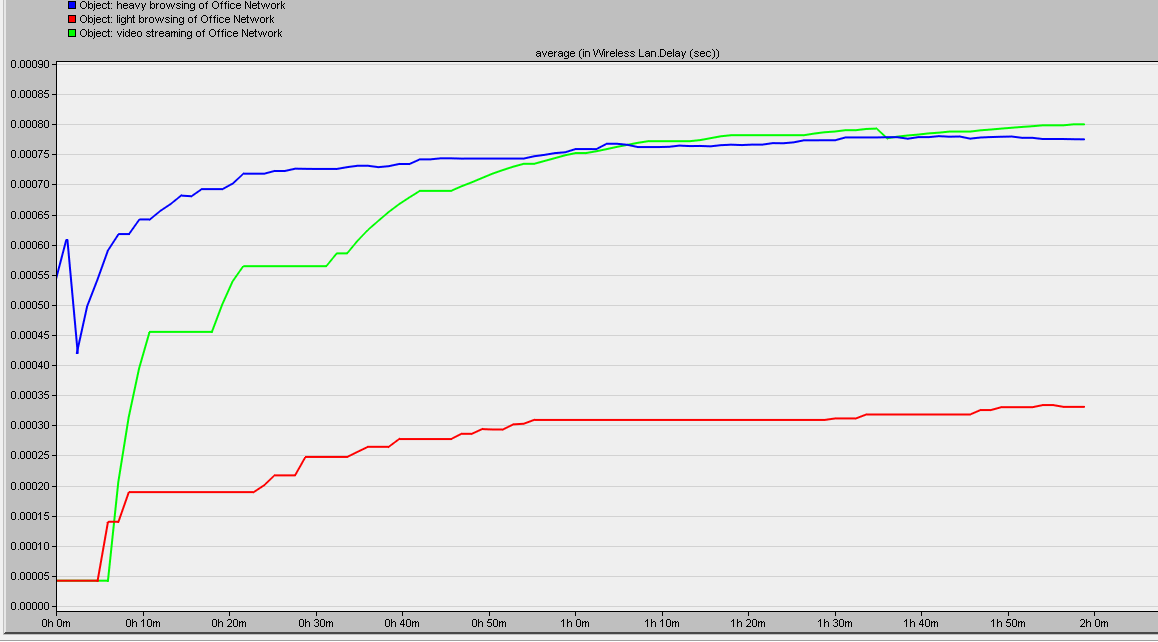
\includegraphics[scale=0.35]{Figures/amantianrenamed/Scenario1ver.png}
	\caption[Scenario 1: comparison of average delay]{Comparison of average delay of light browsing, heavy browsing and video streaming}
	\label{subsubsec:1:summary:delay1}
\end{figure}

In Figure \ref{subsubsec:1:summary:delay1}, heavy browsing has a higher average delay than light browsing due to the higher volume of data transferred. However, the average delay of video streaming is pretty close to that of heavy browsing. The possible reason  is that we are simulating under a \gls{WiFi} environment with a very high data rate so that the video streaming will not have as much delay as we assumed.

\subsection{Scenario 2: Effect of using different video streaming resolutions} \label{subsec:riverbed:2}
\subsubsection{Topology} \label{subsubsec:2:topo}
The wireless LAN parameters, such as data rate and link between router and server, from scenario 1 in Subsection \ref{subsec:riverbed:1} are retained. The range between the router and the two YouTube video nodes remains unchanged. The YouTube video streaming \gls{HTTP} video browsing application is retained because YouTube uses \gls{HTTP} and \gls{TCP} protocols for video streaming as found earlier in the literature review in Subsection \ref{subsec:background:video}. Figure \ref{fig:2:topo} illustrates the topology employed for our second scenario simulations.

\begin{figure}[H]
	\centering
	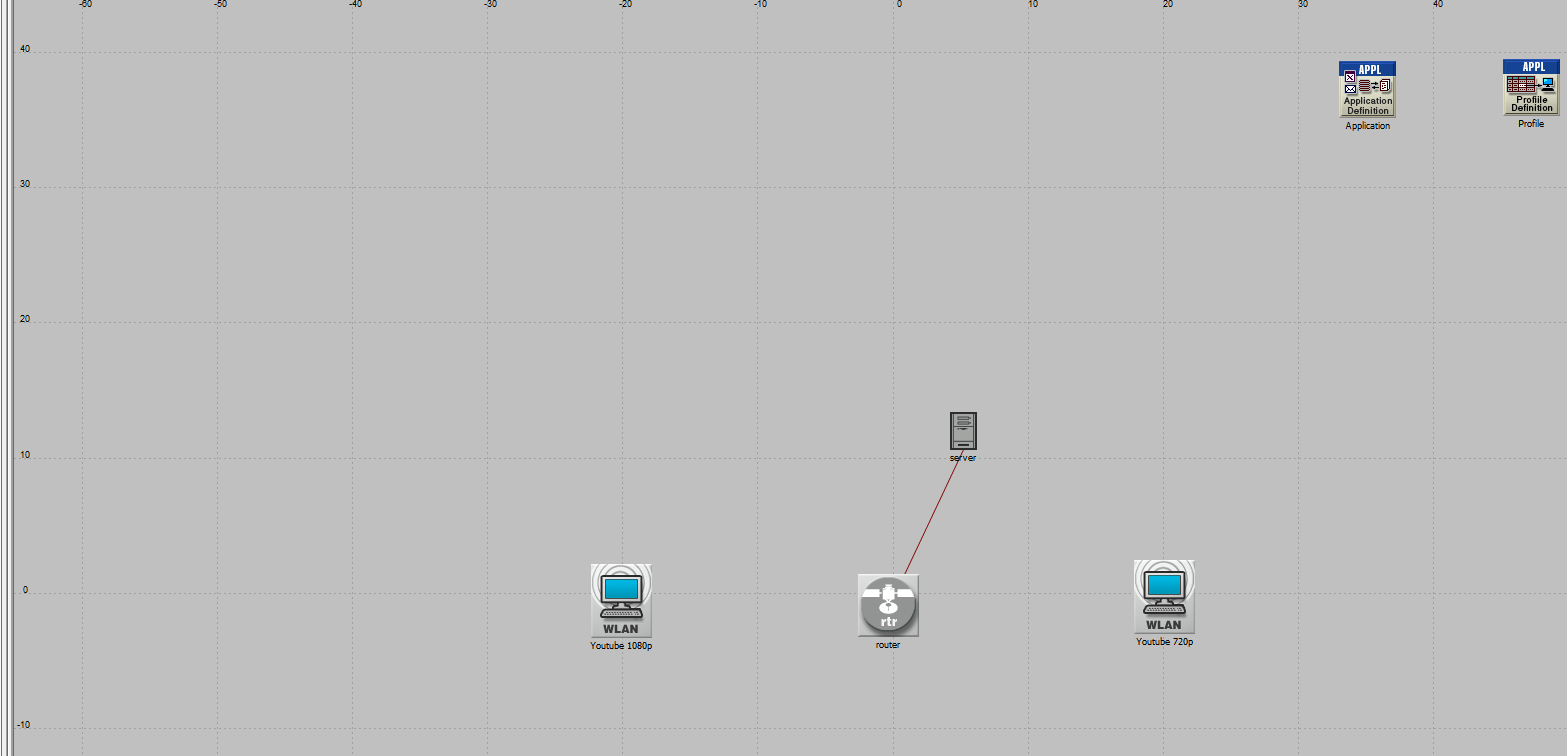
\includegraphics[scale=0.3]{Figures/amantianrenamed/Scenario2Topology.png}
	\caption{Scenario 2: topology}
	\label{fig:2:topo}
\end{figure}

We will also use the YouTube application node for the next few scenarios in this project. YouTube 1080p and 720p use video codec H-264 and the average encoding speed of H-264 is between $24~\mathrm{fps}$ (frames per second) to $30~\mathrm{fps}$.

We can calculate the page inter-arrival time for both YouTube 1080p and 720p by using the frame rate, which are $30~\mathrm{fps}$ for 1080p and $24~\mathrm{fps}$ for 720p. For our simulation, the page inter-arrival time of 1080p is set between $0.0333333~\mathrm{s}$ and $0.0666666~\mathrm{s}$, the page inter-arrival time of 720p is set between $0.0266667~\mathrm{s}$ and $0.0533333~\mathrm{s}$. The page size of both 720p and 1080p are set as short video which is approximately 10000 to 350000 bytes.

Figures \ref{fig:2:http:720p} and \ref{fig:2:http:1080p} show the \gls{HTTP} tables for YouTube 720p and 1080p respectively.
\begin{figure}[H]
	\centering
	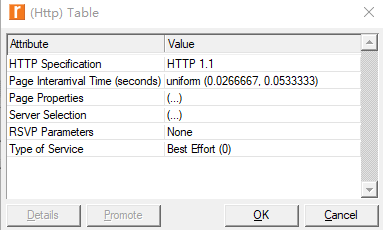
\includegraphics[scale=0.55]{Figures/amantianrenamed/Scenario2YouTube720phttptable.png}
	\caption[Scenario 2: YouTube 720p HTTP table]{Scenario 2: YouTube 720p \gls{HTTP} table}
	\label{fig:2:http:720p}
\end{figure}

\begin{figure}[H]
	\centering
	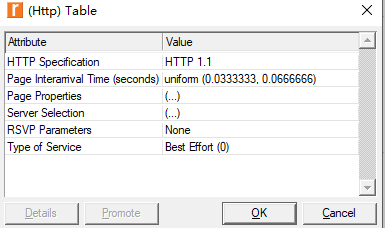
\includegraphics[scale=0.6]{Figures/amantianrenamed/Scenario21080phttpable.png}
	\caption[Scenario 2: HTTP table for YouTube 1080p]{Scenario 2: \gls{HTTP} table for YouTube 1080p}
	\label{fig:2:http:1080p}
\end{figure}

Figure \ref{fig:2:obj} shows the object size for YouTube 720p and 1080p.

\begin{figure}[H]
	\centering
	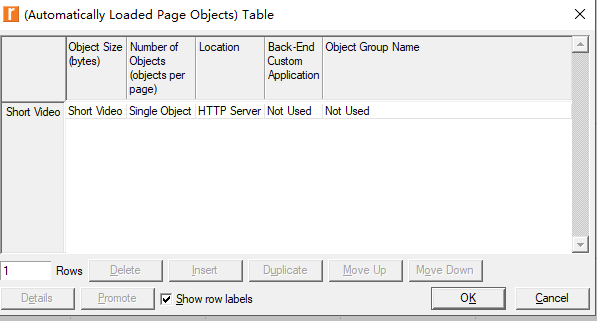
\includegraphics[scale=0.55]{Figures/amantianrenamed/Scenario2YouTube1080pand720pobjectsize.png}
	\caption{Scenario 2: object size for YouTube 720p and 1080p}
	\label{fig:2:obj}
\end{figure}

\subsubsection{Scenario 2 results}
Figure \ref{fig:2:throughput:720p180p} shows that the throughput of 1080p is more than $10000~\mathrm{bps}$ higher than that of 720p as is expected. This is because YouTube 1080p has a longer page inter-arrival time, therefore its frame rate is higher than that of 720p. 

Usually 1080p has a frame rate of $30~\mathrm{fps}$ and 720p has a frame rate of $24~\mathrm{fps}$. With a higher frame rate, 1080p can show more frames per unit time  than 720p, which explains why its throughput is higher than that of 720p.

\begin{figure}[H]
	\centering
	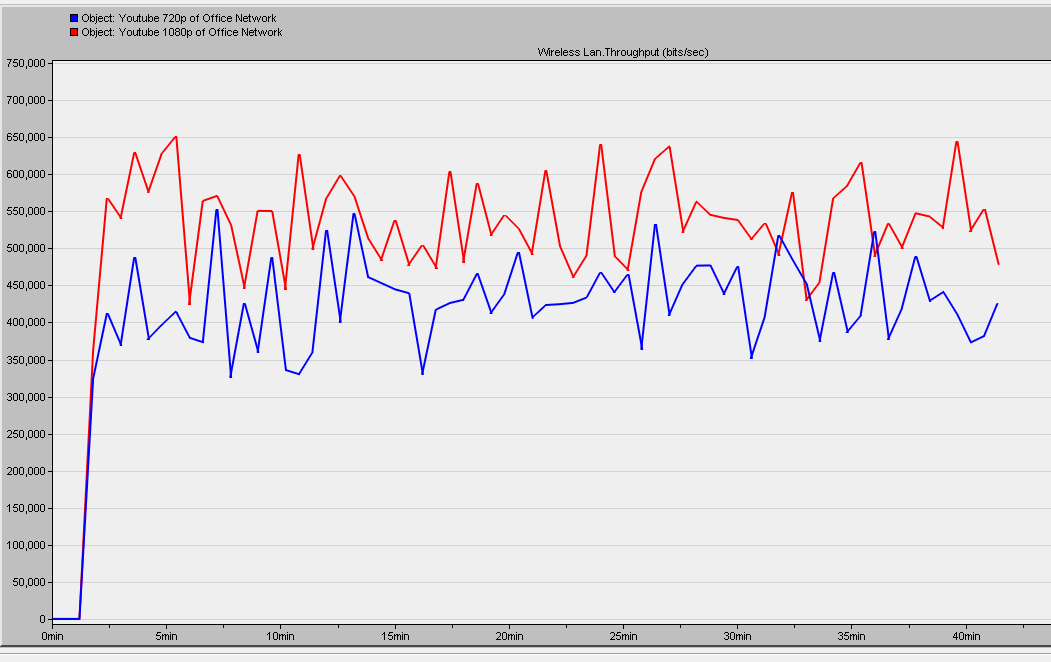
\includegraphics[scale=0.32]{Figures/amantianrenamed/Scenario2Throughputof720pand1080p.png}
	\caption{Scenario 2: Throughput with 720p and 1080p streaming}
	\label{fig:2:throughput:720p180p}
\end{figure}

Figure \ref{fig:2:delay:720p180p} shows that the delay of 1080p is higher than that of 720p. This is expected, because the delay is highly dependent on the throughput. Since 1080p has a higher throughput, it also has a higher delay than 720p.

\begin{figure}[H]
	\centering
	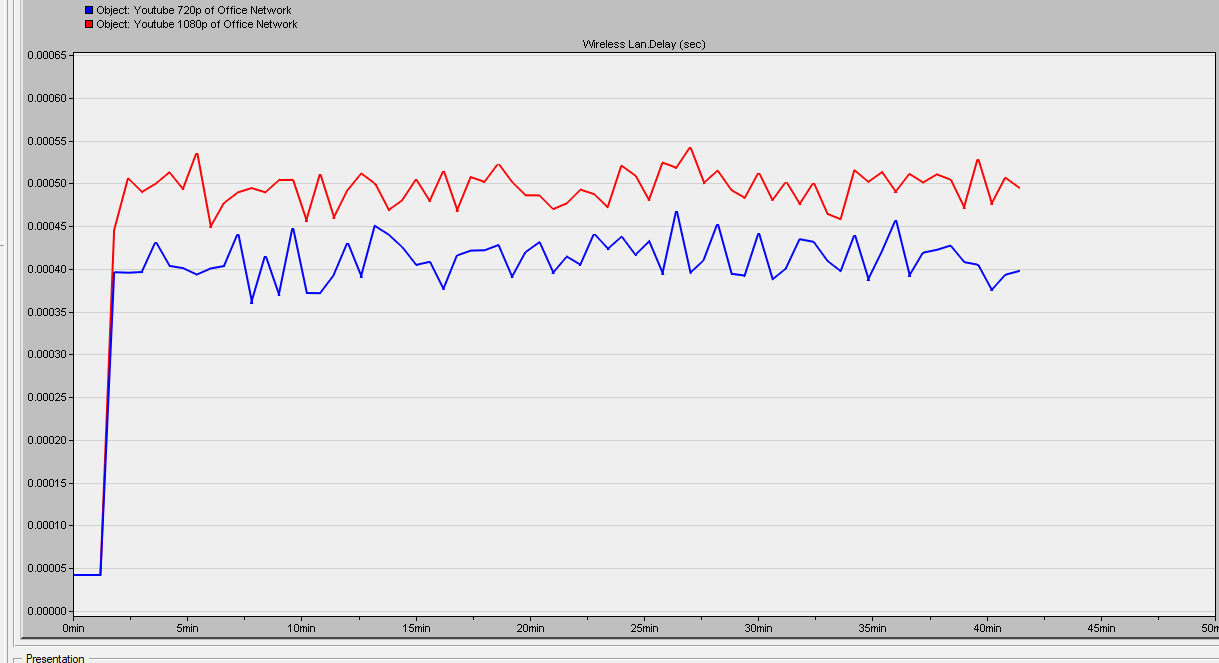
\includegraphics[scale=0.31]{Figures/amantianrenamed/Scenario2Delayof720pand1080p.png}
	\caption{Scenario 2: Delay with 720p and 1080p streaming}
	\label{fig:2:delay:720p180p}
\end{figure}

As can be seen in Figure \ref{fig:2:traffic:720p180p}, 1080p receives more data traffic than 720p from the server. This is due to YouTube 1080p having a higher frame rate. Therefore the server needs to transfer more data per unit time to the streaming client requesting the 1080p video.

\begin{figure}[H]
	\centering
	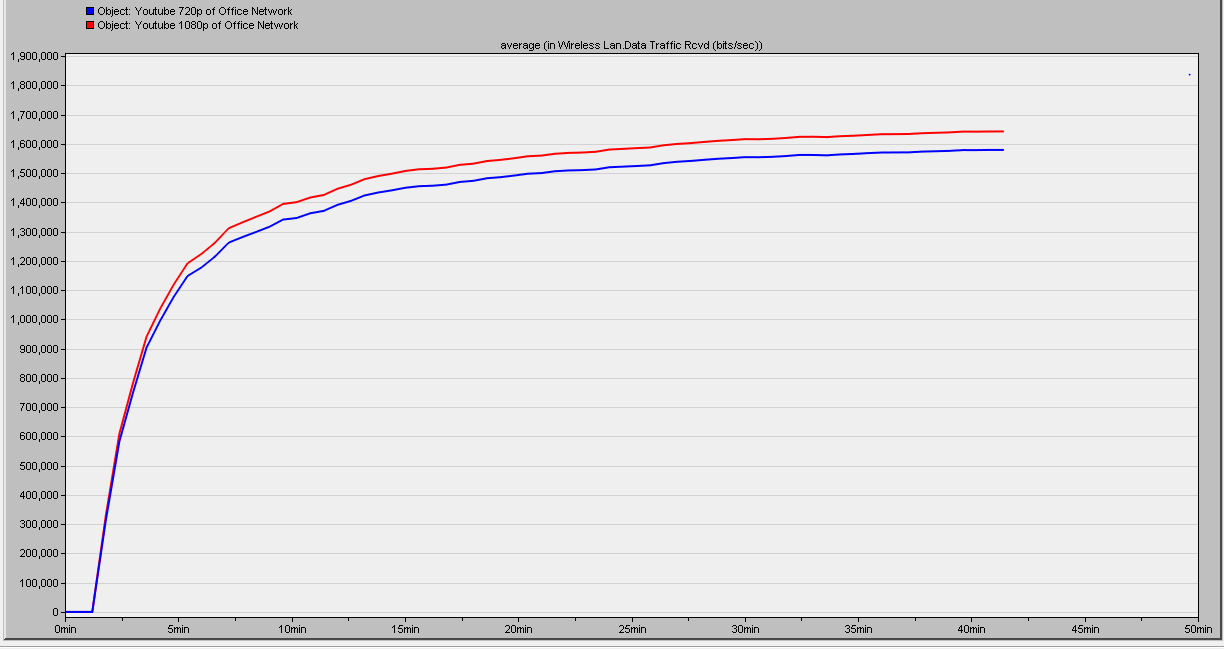
\includegraphics[scale=0.35]{Figures/amantianrenamed/Scenario2Averagedatatrafficreceivedof720pand1080p.png}
	\caption{Scenario 2: Data traffic received with 720p and 1080p streaming}
	\label{fig:2:traffic:720p180p}
\end{figure}

\subsection{Scenario 3: Effect of frequency band, data rate \& WiFi technology} \label{subsec:riverbed:3}
\subsubsection{Scenario 3 topology}
Scenario 3 investigates three aspects: \begin{itemize}
		\item the impact of the \gls{WiFi} technology employed in Subsection \ref{subsub:3:wifi}.
	\item the effect of the frequency band ($2.4~\mathrm{GHz}$ or $5~\mathrm{GHz}$) employed in Subsection \ref{subsub:3:freq}.
	\item the effect of changing the data rate in Subsection \ref{subsub:3:data}.

\end{itemize}

The topology employed in this scenario is very similar to that used in scenario 1 in Subsection \ref{subsec:riverbed:1}, with the only difference being substituting the video streaming node in scenario 1 by the YouTube 1080p node from scenario 2 in Subsection \ref{subsec:riverbed:2}. Figure \ref{fig:3:topo} shows the topology implemented in scenario 3.

\begin{figure}[H]
	\centering
	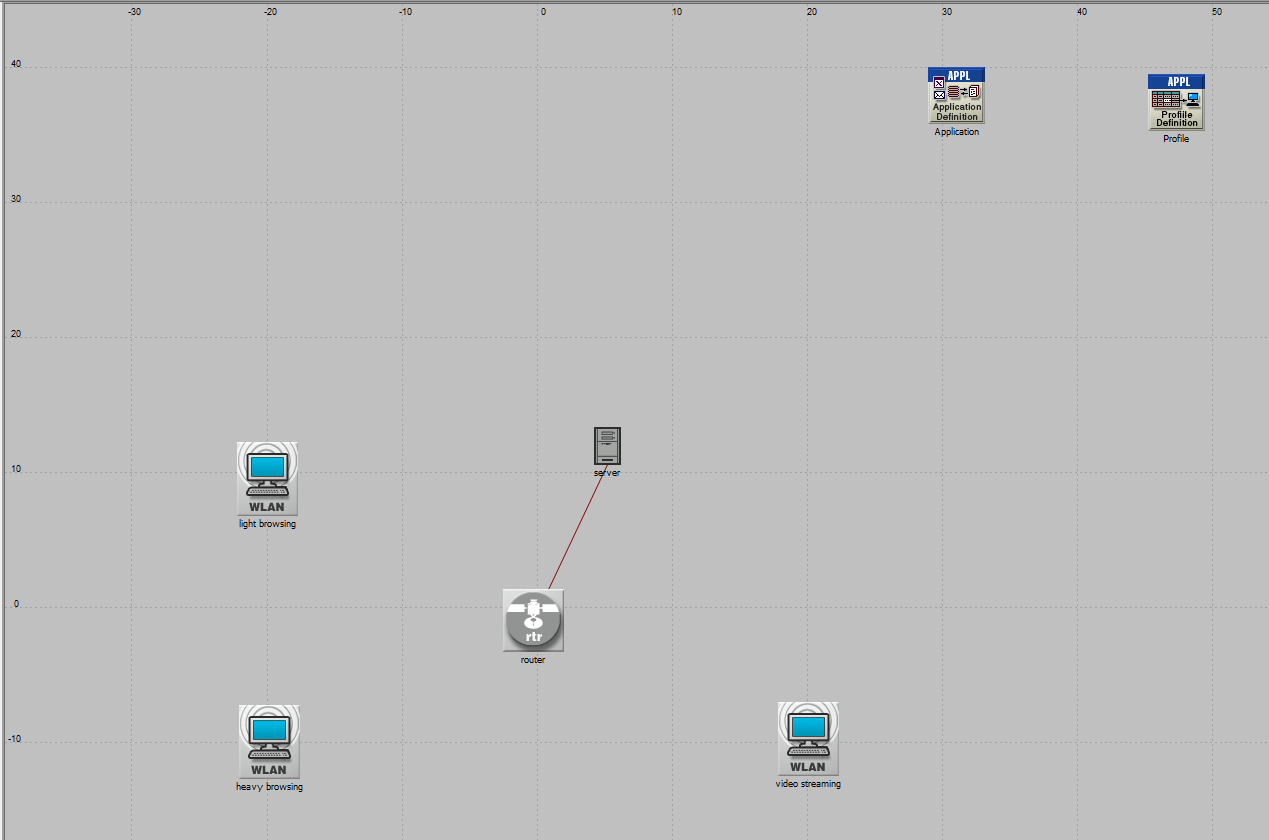
\includegraphics[scale=0.3]{Figures/amantianrenamed/Scenario3Topology.png}
	\caption[Topology employed for Scenario 3]{Topology employed for Scenario 3: A \gls{WLAN} client streams videos at 1080p.}
	\label{fig:3:topo}
\end{figure}

\subsubsection{Impact of WiFi technology} \label{subsub:3:wifi}
To study the impact of the specific \gls{WiFi} technology used, we chose \gls{IEEE802}g operating with a data rate of $24~\mathrm{Mbps}$ and \gls{IEEE802}n with a data rate of $26~\mathrm{Mbps}$ since their data rates are arguably very similar to each other. Figure \ref{fig:3:1} shows the average throughput achieved with this pair of \gls{WiFi} technologies. The average throughput of \gls{IEEE802}n is higher than that of \gls{IEEE802}g by more than $60000~\mathrm{bps}$.

\begin{figure}[H]
	\centering
	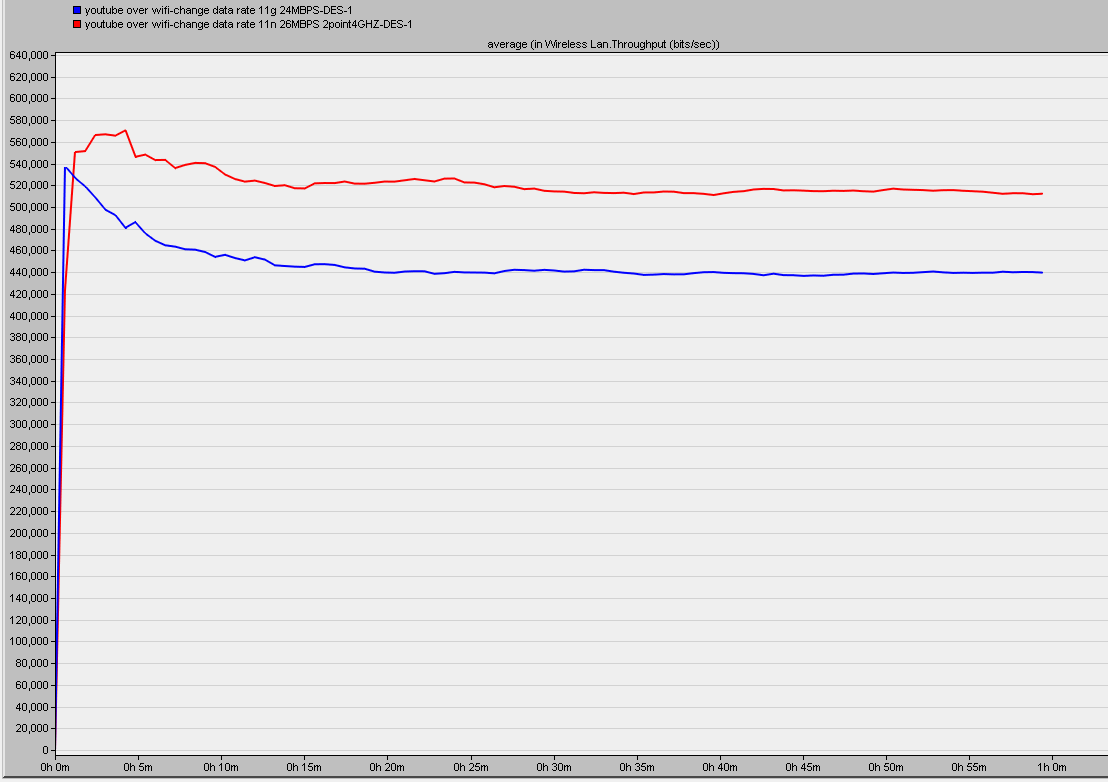
\includegraphics[scale=0.28]{Figures/amantianrenamed/Scen3AveThroughofg24Mn26M.png}
	\caption[Scenario 3: average throughput according to the WiFi technology used]{Scenario 3: Average throughput with \gls{IEEE802}g at $24~\mathrm{Mbps}$ (blue graph) and \gls{IEEE802}n at $26~\mathrm{Mbps}$ (red graph).}
	\label{fig:3:1}
\end{figure}

Figure \ref{fig:3:2} shows the average delay with this pair of \gls{WiFi} technologies. The average delay of \gls{IEEE802}g is higher than that of \gls{IEEE802}n by more than $0.0008~\mathrm{s}$.

\begin{figure}[H]
	\centering
	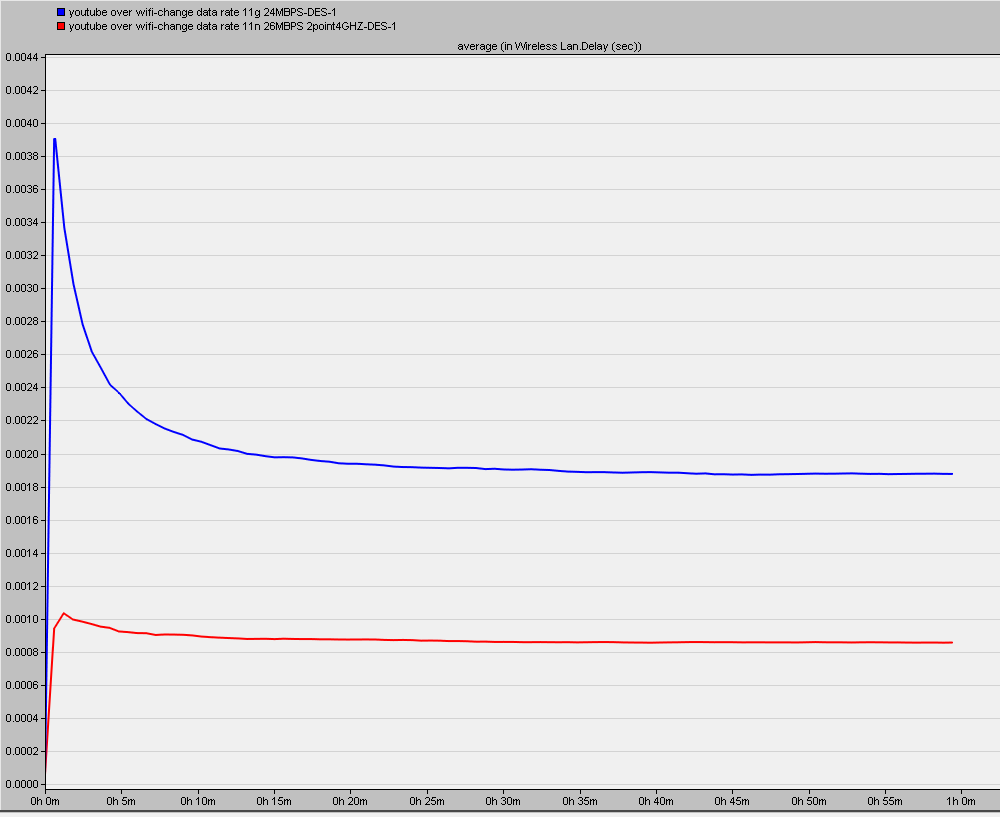
\includegraphics[scale=0.29]{Figures/amantianrenamed/Scenario3AverageDelayof80211g24Mbpsand8021126Mbps.png}
	\caption[Scenario 3: average delay according to the WiFi technology used]{Scenario 3: Average delay with \gls{IEEE802}g at $24~\mathrm{Mbps}$ (blue graph) and \gls{IEEE802}n at $26~\mathrm{Mbps}$ (red graph).}
	\label{fig:3:2}
\end{figure}

The improved throughput and delay experienced with \gls{IEEE802}n is more likely thanks to its higher data rate of $26~\mathrm{Mbps}$ than to any inherent superiority in technology over \gls{IEEE802}g.

\subsubsection{Effect of frequency band} \label{subsub:3:freq}
To investigate the effect of frequency band, we employed the dual-band capable \gls{IEEE802}n. We used the same data rate of $26~\mathrm{Mbps}$ and physical characteristics with the YouTube 1080p node. 

Figure \ref{fig:3:3} shows the average throughput experienced in the two frequency bands. Since the two graphs are very
close to each other, we can conclude that within the parameters of our experiment, the throughput performance is independent of the choice of frequency band.

\begin{figure}[H]
	\centering
	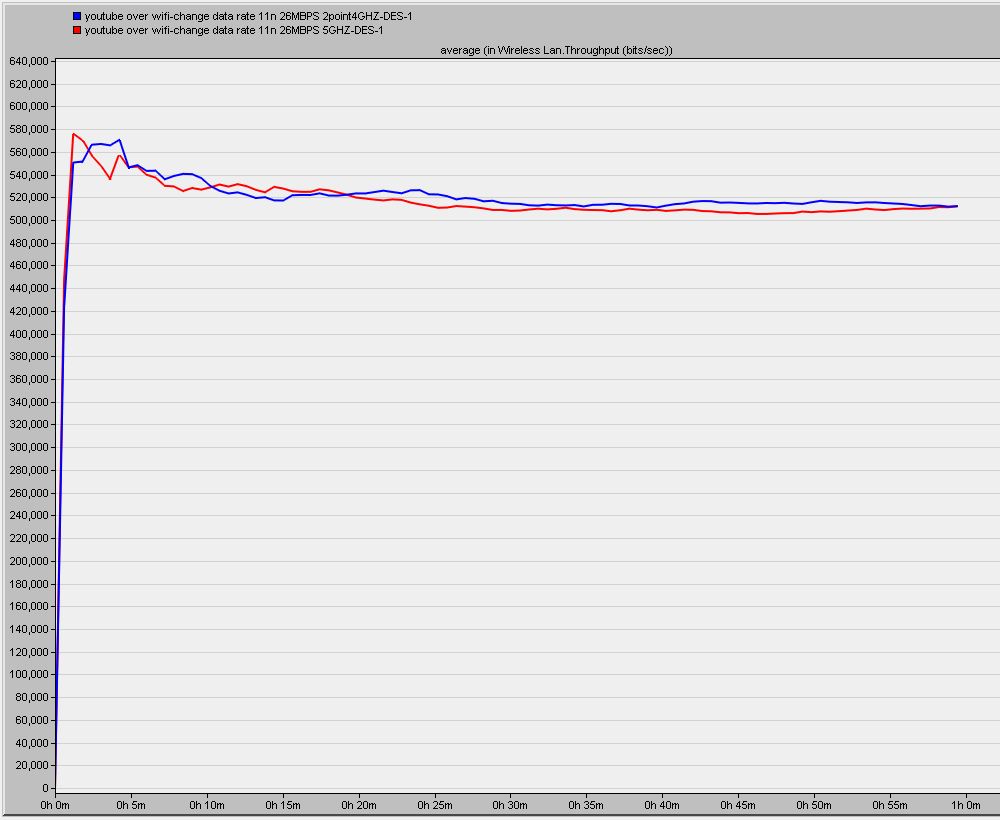
\includegraphics[scale=0.3]{Figures/amantianrenamed/Scenario3AverageThroughputof802.11n26Mbps2.4GHzand802.11n26Mbps5GHz.png}
	\caption[Scenario 3: average throughput according to the frequency band used]{Scenario 3: average throughput of \gls{IEEE802}n at $26~\mathrm{Mbps}$: $2.4~\mathrm{GHz}$ (blue graph) and  $5~\mathrm{GHz}$ (red graph).}
	\label{fig:3:3}
\end{figure}

Figure \ref{fig:3:4} shows the average delay experienced in the two frequency bands. Since the two graphs are very close to each other, we can conclude that within the parameters of our experiment, the delay performance is independent of the choice of frequency band.

\begin{figure}[H]
	\centering
	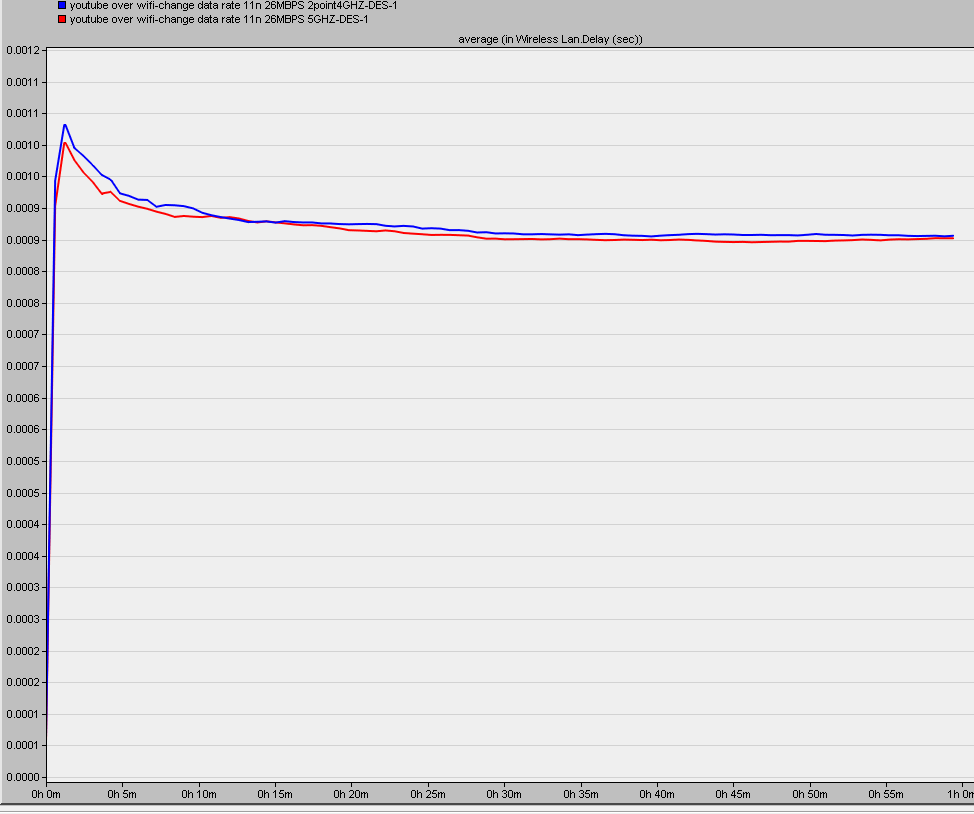
\includegraphics[scale=0.3]{Figures/amantianrenamed/Scenario3Avedelay11n2624GHz80211n26Mbps5GHz.png}
	\caption[Scenario 3: average delay according to the frequency band used]{Scenario 3: average delay with \gls{IEEE802}n at $26~\mathrm{Mbps}$: $2.4~\mathrm{GHz}$ (blue graph) and  $5~\mathrm{GHz}$ (red graph).}
	\label{fig:3:4}
\end{figure}

The frequency band chosen does not have a significant effect within the parameters of our experiment because the \gls{WiFi} client was very close to the \gls{WiFi} access point and therefore attenuation effects did not come into play. Furthermore, since there were not a large number of clients sharing the same \gls{WiFi} connection, the client could enjoy the full capacity of the \gls{WiFi} connection.

\subsubsection{Effect of data rate} \label{subsub:3:data}
Finally, we investigate the effect of changing the data rate on the performance experienced by the YouTube 1080p node. We employ the \gls{IEEE802}n standard in the $2.4~\mathrm{GHz}$ band.

Figure \ref{fig:3:5} shows the average throughput experienced with the chosen data rates. As expected, with the higher data rate, the throughput experienced is higher than at the lower data rate.

\begin{figure}[H]
	\centering
	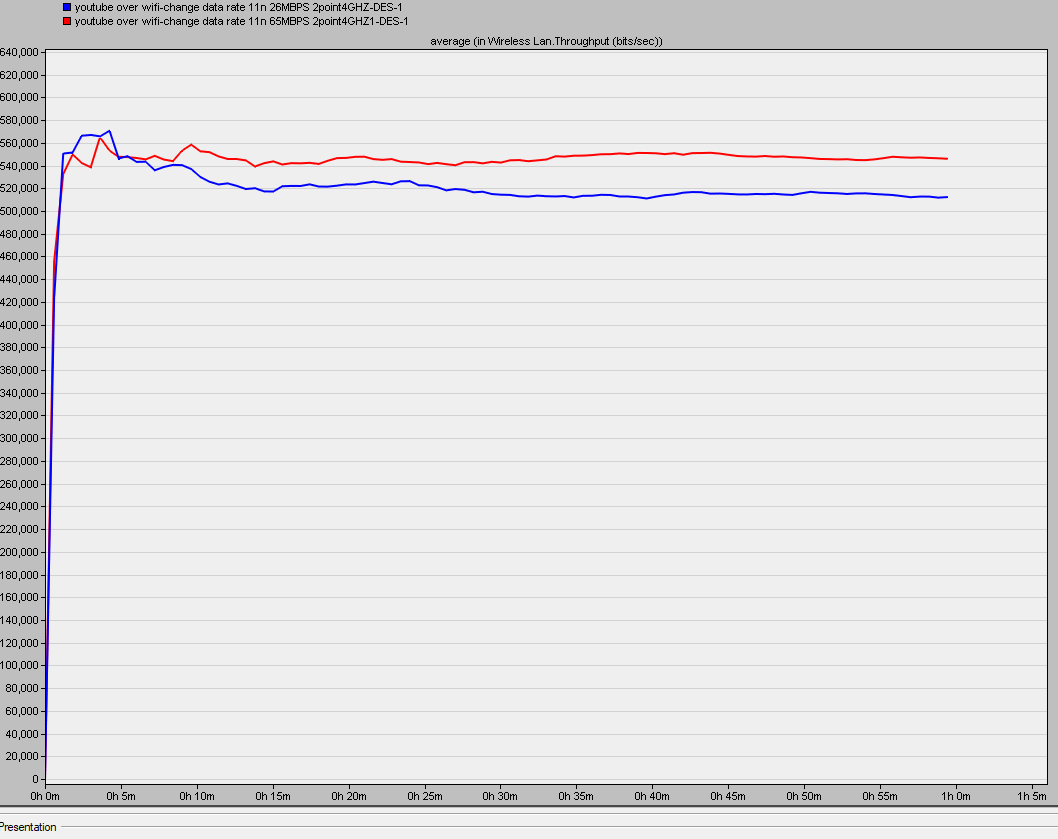
\includegraphics[scale=0.3]{Figures/amantianrenamed/Scenario3AverageThroughputof802.11n26Mbps2.4GHzand802.11n65Mbps2.4GHz.png}
	\caption[Scenario 3: average throughput according to data rate]{Scenario 3: average throughput of \gls{IEEE802}n at $2.4~\mathrm{GHz}$: $26~\mathrm{Mbps}$ (blue graph) and $65~\mathrm{Mbps}$ (red graph). }
	\label{fig:3:5}
\end{figure}

Figure \ref{fig:3:6} shows the average delay experienced with the chosen data rates. The \gls{WiFi} client experiences more delay at the lower data rate. 
%We suspect that jitter is playing a role in the poorer delay experienced at $65~\mathrm{Mbps}$.

\begin{figure}[H]
	\centering
	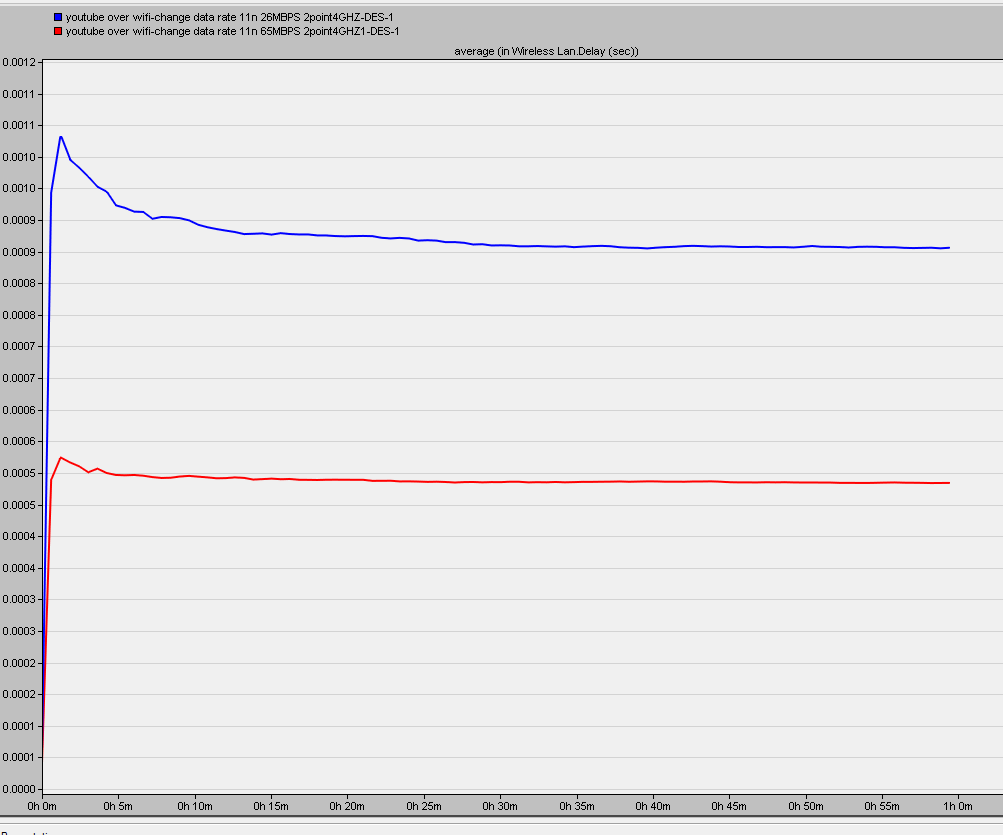
\includegraphics[scale=0.3]{Figures/amantianrenamed/Scenari3AveDelayn26M2.4GHzn65Mbps4GHz.png}
	\caption[Scenario 3: average delay according to data rate]{Scenario 3: average delay of \gls{IEEE802}n at $2.4~\mathrm{GHz}$: $26~\mathrm{Mbps}$ (blue graph) and $65~\mathrm{Mbps}$ (red graph). }
	\label{fig:3:6}
\end{figure}

\subsection{Scenario 4: Effect of varying the range to the WiFi access point} \label{subsec:riverbed:4}
Scenario 4 employs the same \gls{WLAN} parameter settings as scenario 3 in Subsection \ref{subsec:riverbed:3}, except that the YouTube 1080p node was moved almost 200 meters away from the router. The objective is to investigate the effect of changing the range to the \gls{WiFi} access point on the performance of the 1080p node. Physical characteristics, data rate and \gls{IEEE802} technology employed are varied in this set of experiments. The range from the user to the router in Scenario 4 is exaggerated on purpose to better show the impact of the range.

\begin{figure}[H]
	\centering
	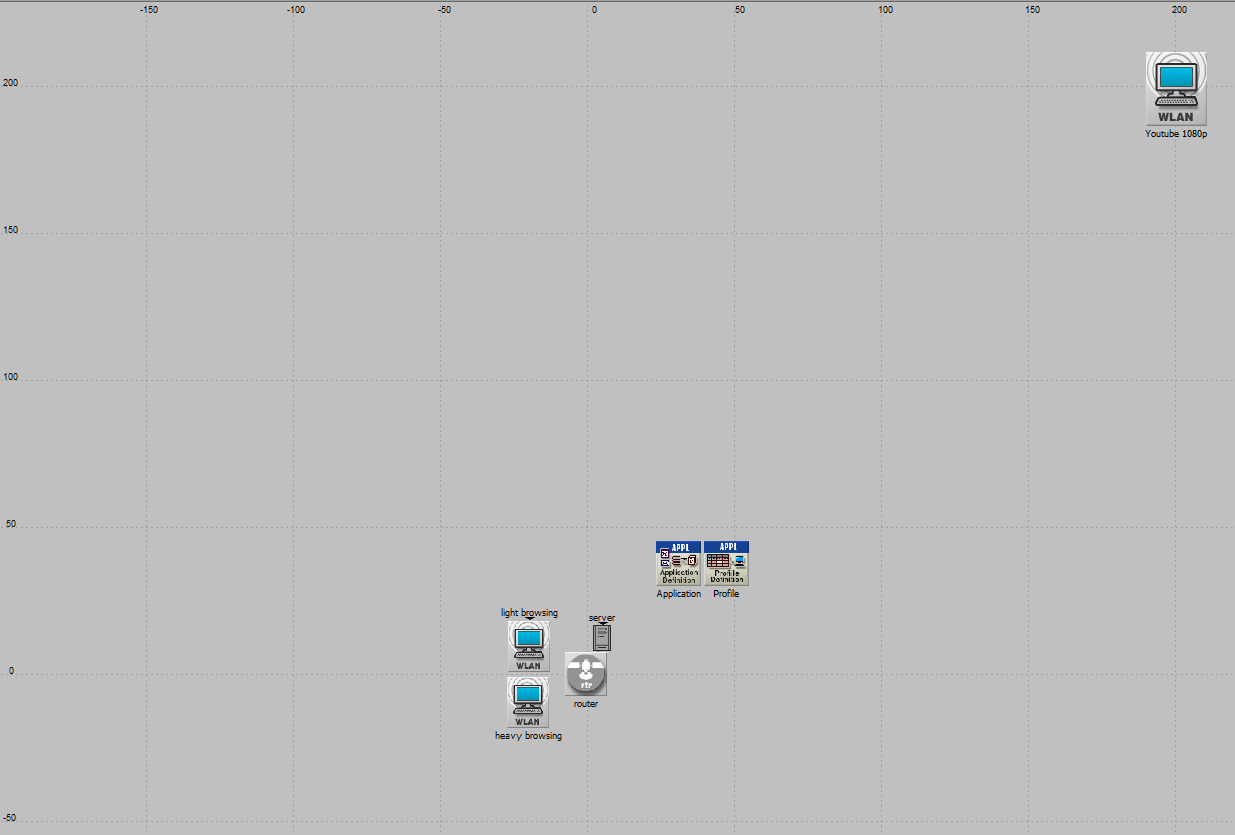
\includegraphics[scale=0.278]{Figures/amantianrenamed/scenario4topo.png}
	\caption{Scenario 4: topology}
	\label{fig:4:1}
\end{figure}

Figure \ref{fig:4:2} shows the throughput achieved at data rates of $39~\mathrm{Mbps}$ (blue graph) and $65~\mathrm{Mbps}$ (red graph) when employing \gls{IEEE802}n in the $2.4~\mathrm{GHz}$ band. The throughput dropped to zero in the $65~\mathrm{Mbps}$ case for some unexplained reason. We suspect that we made a mistake in our simulation but we have not been able to debug this issue.

\begin{figure}[H]
	\centering
	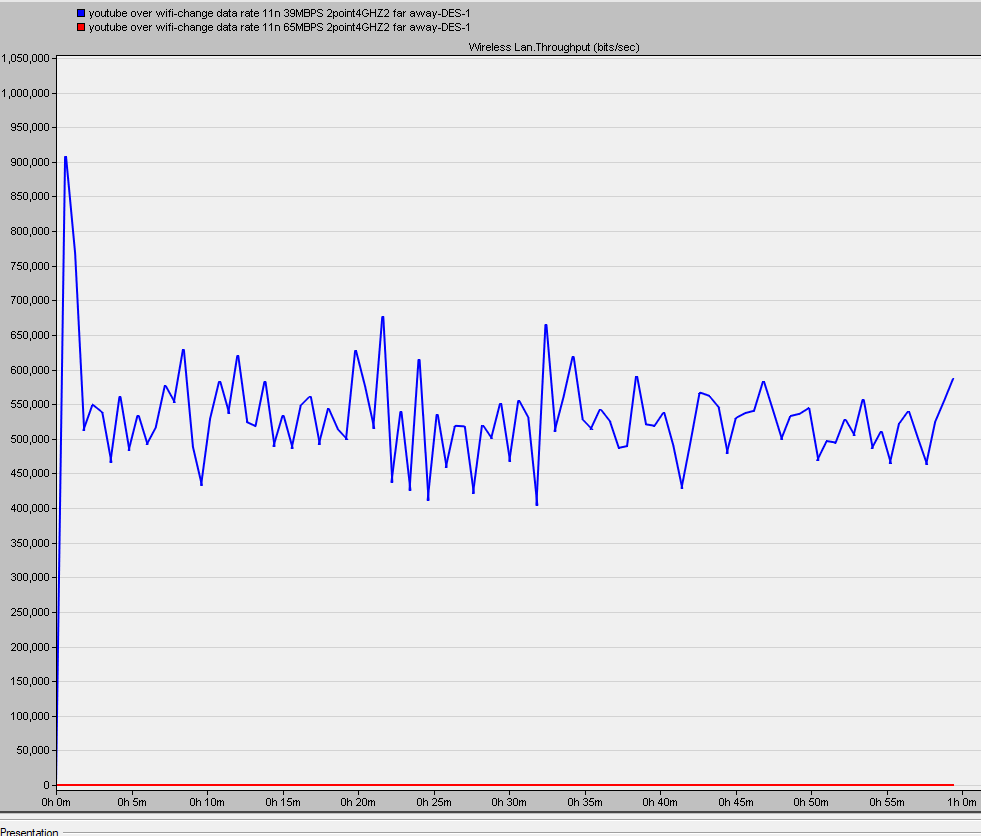
\includegraphics[scale=0.3]{Figures/amantianrenamed/Scenario4Throughputof802.11n39Mbps.4GHzand802.11n65Mbps2.4GHz.png}
	\caption[Scenario 4: throughput at data rates of $39~\mathrm{Mbps}$ and $65~\mathrm{Mbps}$]{Scenario 4: throughput with \gls{IEEE802}n at $2.4~\mathrm{GHz}$: data rate of $39~\mathrm{Mbps}$ (blue graph) and $64~\mathrm{Mbps}$ (red graph).}
	\label{fig:4:2}
\end{figure}

We retained \gls{IEEE802}n operating in the $2.4~\mathrm{GHz}$ band as technology and investigated the effect of changing the data rate from $39~\mathrm{Mbps}$ to $26~\mathrm{Mbps}$. Figure \ref{fig:4:3} shows the average throughput graphs while Figure \ref{fig:4:4} shows the corresponding average delay graphs.

\begin{figure}[H]
	\centering
	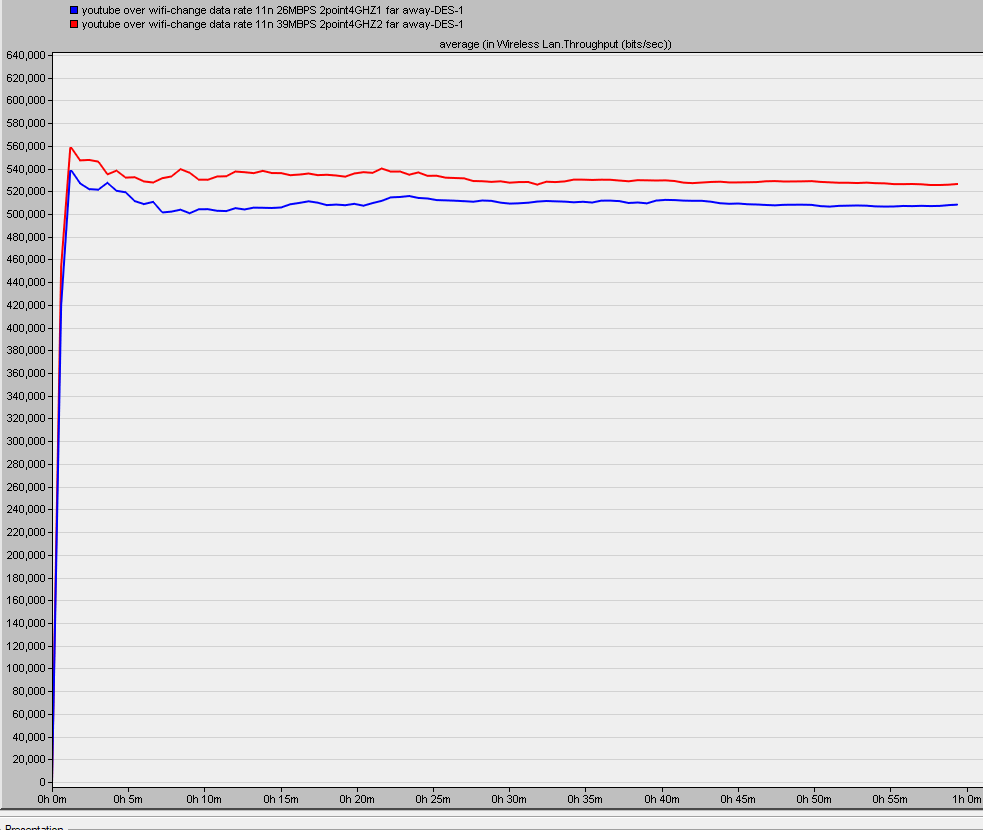
\includegraphics[scale=0.3]{Figures/amantianrenamed/Scenario4AveThroughputof39Mbpsand26Mbps.png}
	\caption[Scenario 4: average throughput at data rates of $26~\mathrm{Mbps}$ and $39~\mathrm{Mbps}$]{Scenario 4: Average \gls{WLAN} throughput with \gls{IEEE802}n at $2.4~\mathrm{GHz}$: data rate of $26~\mathrm{Mbps}$ (blue graph) and $39~\mathrm{Mbps}$ (red graph).}
	\label{fig:4:3}
\end{figure}

As can be seen in Figure \ref{fig:4:3}, the throughput experienced by the YouTube 1080p node remains acceptable when the data rate chosen is lower than $65~\mathrm{Mbps}$ which was found to be problematic in Figure \ref{fig:4:2}. With the streaming client node being located further away from the router, the higher data rate $39~\mathrm{Mbps}$ of the \gls{WiFi} connection leads to higher throughput (c.f. Figure \ref{fig:4:3}) and lower delay (c.f. Figure \ref{fig:4:4}), as expected. With a higher data rate (as long as it is lower than $65~\mathrm{Mbps}$), the streaming client enjoys better \gls{QoS} even when located further away from the \gls{WiFi} access point.

\begin{figure}[H]
	\centering
	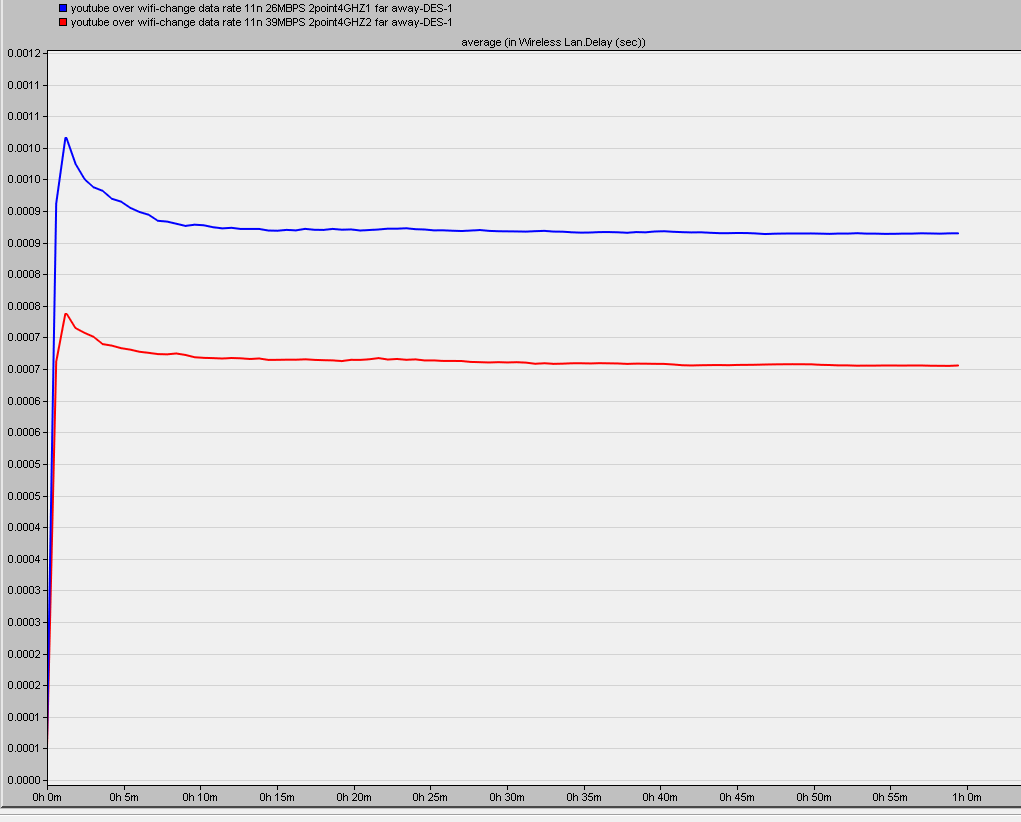
\includegraphics[scale=0.3]{Figures/amantianrenamed/Scenario4Avedelayof39Mbpand26Mbps.png}
	\caption[Scenario 4: average delay at data rates of $26~\mathrm{Mbps}$ and $39~\mathrm{Mbps}$]{Scenario 4: Average \gls{WLAN} delay with \gls{IEEE802}n at $2.4~\mathrm{GHz}$: data rate of $26~\mathrm{Mbps}$ (blue graph) and $39~\mathrm{Mbps}$ (red graph).}
	\label{fig:4:4}
\end{figure}

We then investigated the effect of increasing the range when the \gls{WLAN} operates in either of the two frequency bands supported by \gls{IEEE802}n.

Figure \ref{fig:4:5} shows the average throughput achieved in both frequency bands of \gls{IEEE802}n operating at a data rate of $26~\mathrm{Mbps}$.

\begin{figure}[H]
	\centering
	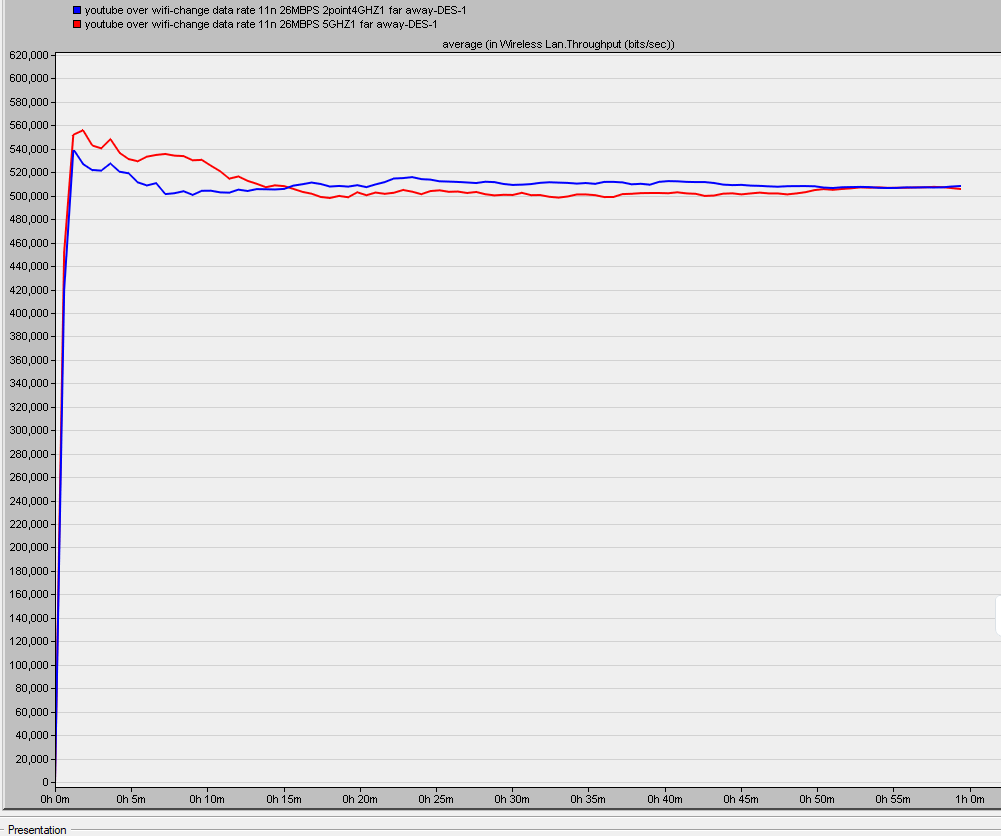
\includegraphics[scale=0.3]{Figures/amantianrenamed/Scenario4AveThroughpuof26Mbps2.4GHzand26Mbps5GHz.png}
	\caption[Scenario 4: average throughput at $26~\mathrm{Mbps}$ in two frequency bands]{Scenario 4: average throughput in the $2.4~\mathrm{GHz}$ band (blue graph) and $5~\mathrm{GHz}$ (red graph) with a data rate of $26~\mathrm{Mbps}$}
	\label{fig:4:5}
\end{figure}

As can be seen in Figure \ref{fig:4:5}, the streaming client enjoys similar average throughputs in either of the frequency bands. It is important to note that the number of \gls{WiFi} clients was not a limiting factor to the performance in our simulation, therefore the higher host accommodation capacity of the $5~\mathrm{GHz}$ band has no impact in our simulation.

Figure \ref{fig:4:6} shows the average delay achieved in both frequency bands of \gls{IEEE802}n operating at a data rate of $26~\mathrm{Mbps}$.

\begin{figure}[H]
	\centering
	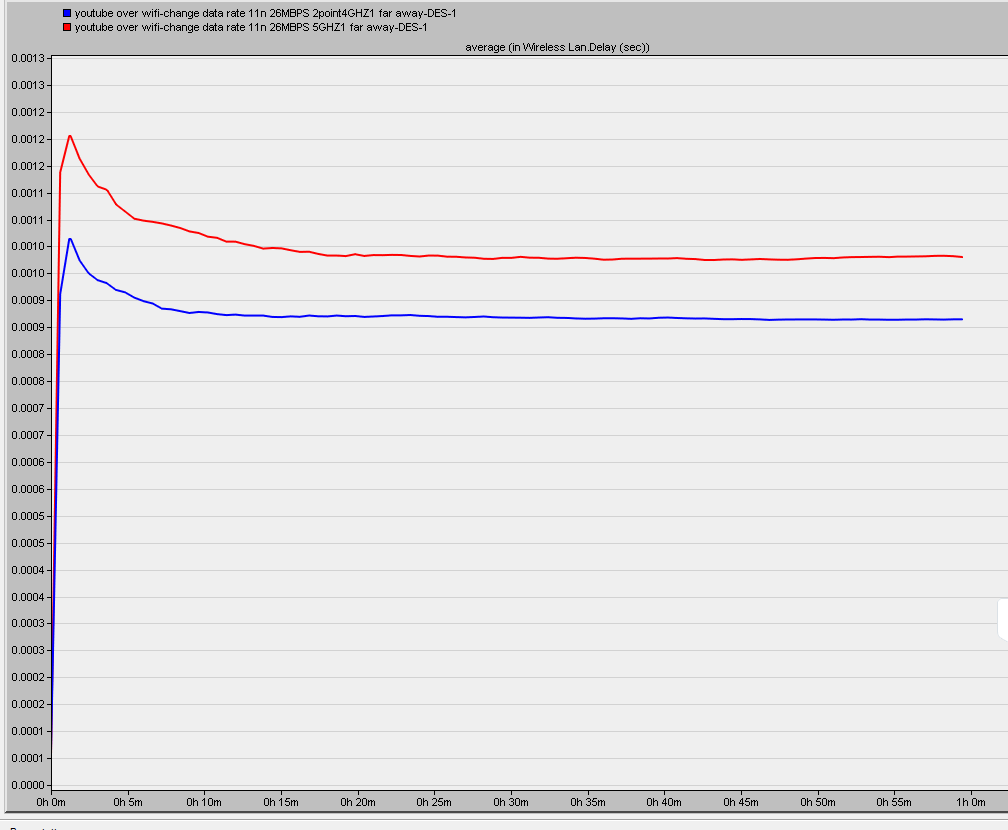
\includegraphics[scale=0.3]{Figures/amantianrenamed/Scenario4Avedelayof802.11n26Mbps2.4GHzand26Mbps5GHz.png}
	\caption[Scenario 4: average delay at $26~\mathrm{Mbps}$ in two frequency bands]{Scenario 4: average delay in the $2.4~\mathrm{GHz}$ band (blue graph) and $5~\mathrm{GHz}$ (red graph) with a data rate of $26~\mathrm{Mbps}$}
	\label{fig:4:6}
\end{figure}

As can be seen in Figure \ref{fig:4:6}, when the client streams in the $5~\mathrm{GHz}$ band, it experiences a higher average delay than operating in the $2.4~\mathrm{GHz}$ band in this particular case where the client is further away from the router. This is explained by the fact that the power of radio signals attenuate more significantly in higher frequency bands (such as the $5~\mathrm{GHz}$ band) than in lower frequency bands (such as the $2.4~\mathrm{GHz}$ band). 
Furthermore, objects of similar size to the wavelength of $6~\mathrm{cm}$ of $5~\mathrm{GHz}$ \gls{WiFi} readily absorb 
it, as was discussed in Subsection \ref{subsec:background:ieee802}. These phenomena are observed when the range to the transmitter (i.e. the \gls{WiFi} access point) is higher but not when the range is negligible as we found earlier in Subsection \ref{subsub:3:freq}.

Finally, we compared the average data dropped in the current scenario (higher range between the client and router) under various conditions to bring together the different scenarios we investigated.

Figure \ref{fig:4:7} shows that when \gls{IEEE802}g is used, the client experiences much smaller average data dropped than when any other \gls{IEEE802}n case is used. When located further away from the router, the YouTube 1080p streaming node enjoys better \gls{QoS} with \gls{IEEE802}g than with \gls{IEEE802}n. This result comes with the caveat that the streaming client did not have to share the \gls{WiFi} connection with a large number of co-hosts.

\begin{figure}[H]
	\centering
	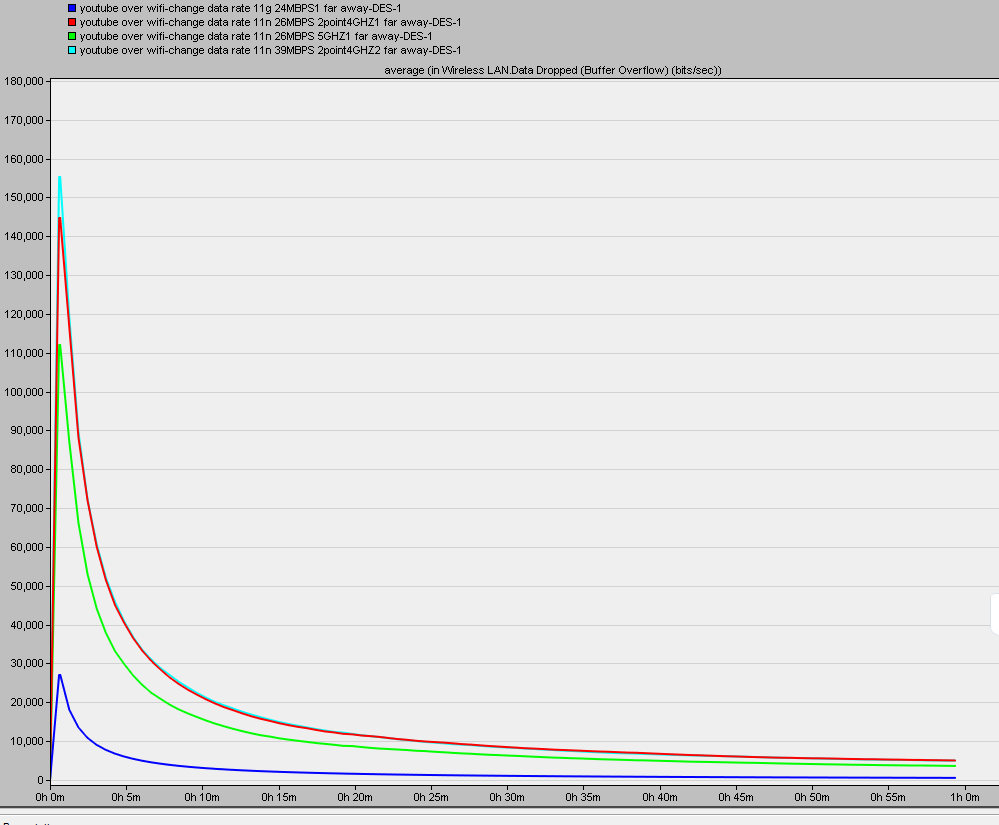
\includegraphics[scale=0.3]{Figures/amantianrenamed/Scenario4Averagedatadropped.png}
	\caption[Scenario 4: average data dropped under various conditions]{Scenario 4: average data dropped under various conditions: \gls{IEEE802}g with a data rate of $24~\mathrm{Mbps}$ (blue graph), \gls{IEEE802}n ($2.4~\mathrm{GHz}$) at $26~\mathrm{Mbps}$ (red graph), \gls{IEEE802}n ($5~\mathrm{GHz}$) at $26~\mathrm{Mbps}$ (green graph) and \gls{IEEE802}n ($2.4~\mathrm{GHz}$) at $39~\mathrm{Mbps}$ (pale blue graph)}
	\label{fig:4:7}
\end{figure}

\section{Summary} \label{sec:summary}
This chapter has discussed at length the design and simulation of experiments conducted in this project. It has described preliminary investigations such as pinging YouTube in Section \ref{sec:simul:ping} and studying a YouTube streaming trace with Wireshark \ref{sec:simul:wireshark}. Based on these findings, the discussion moved to the experiments done using Riverbed Modeler.

The conclusions drawn on the work presented in this chapter are elaborated on in Chapter \ref{chapter:discussion}.
